%%%%%%%%%%%%%%%%%%%%%%%%%%%%%
\documentclass{article}

% Language setting
% Replace `english' with e.g. `spanish' to change the document language
\usepackage[english]{babel}

% Set page size and margins
% Replace `letterpaper' with`a4paper' for UK/EU standard size
\usepackage[letterpaper,top=2cm,bottom=2cm,left=3cm,right=3cm,marginparwidth=1.75cm]{geometry}

% Useful packages
\usepackage{amsmath}
\usepackage{graphicx}
\usepackage[colorlinks=true, allcolors=blue]{hyperref} % Setup hyperlinks to blue
\usepackage{amssymb}
\usepackage{algorithm2e}
\usepackage{float} % Make algorithm appear in correct location
\newtheorem{theorem}{Theorem}
\usepackage{amssymb} % Used for \triangleq
% \usepackage{pxfonts} % optional font change
% \usepackage[LGRgreek]{mathastext} % Option to remove italics from all equations

% New commands
% \newcommand{\R}{\ensuremath{\mathbb{R}}}

%%%%%%%%%%%%%%%%%%%%%%%%%%%%%
\begin{document}

% Chapters
\title{Comparison of Quaternion and Invariant Extended Kalman Filter}
\author{Jack Sonstegard}

\maketitle

\section{Introduction}
%%%%%%%%%%%%%%%%%%%%%%%%%%%%%
% Start of introduction
\subsection{Purpose}

The purpose of this project is to explore advanced state estimation techniques that are applicable to the Aerospace industry. Specifically, I wanted to compare a Quaternion Extended Kalman Filter (QEKF) to a Invariant Extended Kalman Filter (InEKF). Both filters provide unique methods to tackle the problem of nonlinear state estimation in systems involving attitude. This report serves as a resource for background information on the formulation of each filter and provides a Monte Carlo simulation comparing each filter.

\subsection{Outline}

This document begins with a background on how IMU and GPS measurements can be modeled. The essential background needed to understand both the QEKF and InEKF filters is then provided including derivation steps for the error dynamics. Building on this foundation, the filters are applied in a simulation using drone data from the Mid-Air Dataset, which includes accelerometer and gyroscope measurements \cite{Fonder2019MidAir}, along with GPS position data. A Monte Carlo analysis reveals that when using just a GPS position measurement both the InEKF and QEKF suffer from unobservability in the bias states. However, quicker convergence to a solution is seen across Monte Carlos in the InEKF.

\subsection{Disclaimer}

This document is not intended to be a comprehensive guide to each filter but is intended to provide enough background such that someone could start experimenting with each filter assuming they already have some background in Kalman Filtering. Throughout this document different references will be cited, however, there are two main papers that helped me learn the most about each filter. The first is the paper by Joan Sol{\`{a}} titled "Quaternion kinematics for the error-state Kalman Filter" \cite{Quaternion_Kinematics_for_the_Error-state_EKF}. This paper gives detailed explanation of quaternion definitions, conventions, and their use in filtering. The second paper is by Ross Hartley et al., titled "Contact-Aided Invariant Extended Kalman Filtering for Robot State Estimation" \cite{Contact-Aided_Invarant_EKF}. This paper was my original inspiration for starting this project. In this paper, the InEKF is derived in multiple forms and necessary background is provided for Lie groups and Lie algebras.

%%%%%%%%%%%%%%%%%%%%%%%%%%%%%
\section{Sensor Modeling}
%%%%%%%%%%%%%%%%%%%%%%%%%%%%%
\subsection{Purpose}
In order to compare the QEKF and InEKF a drone simulation from the Mid-Air Dataset \cite{Fonder2019MidAir} was used which simulated low-altitude drone flights. Using the trajectory of the done, an Inertial Measurement Unit (IMU) containing an accelerometer and gyroscope as well as a GPS receiver and magnetometer were simulated. These sensors provide measurements that are received by each filter and must be correctly modeled by each filter to estimate the drone pose. This section explains how these sensors are modeled in simulation. These models will then be subsequently used in each filter in order to estimate the state of the drone.

\subsection{IMU Continuous Time Model}
The IMU consists of a model for the acceleration, angular rate, and random walk biases. These states are measured in the body frame of the drone. Overall, two coordinate frames will be used in this report. A body frame attached to the drone and a world frame are the initial starting point of the drone trajectory. Both frames use the North, East, and Down (NED) convention. The measured acceleration and angular rate of the drone in the body frame coordinates as well as the model of the biases are defined as
\begin{subequations} \label{eq: measurement model}
    \begin{align}
        \Tilde{a} &= a + b^a + w^a, \quad w^a \sim \mathcal{N}(0_{3,1}, \sigma_{a}^2) \label{eq:accel meas} \\
        \Tilde{\omega} &= \omega + b^{\omega} + w^{\omega}, \quad w^{\omega} \sim \mathcal{N}(0_{3,1}, \sigma_{\omega}^2) \label{eq:omega meas} \\
        \dot{b}^a &= w^{ba}, \quad w^{ba} \sim \mathcal{N}(0_{3,1}, \sigma_{ba}^2) \label{eq:rw bias accel} \\
        \dot{b}^{\omega} &= w^{b\omega}, \quad w^{b\omega} \sim \mathcal{N}(0_{3,1}, \sigma_{b\omega}^2) \label{eq:rw bias omega}
    \end{align}
\end{subequations}
Each variable in the above equations is in $\mathbb{R}^3$ representing a component in the North, East, and Down directions for the respective coordinate frame. In equations \eqref{eq:accel meas} and \eqref{eq:omega meas}, the measured values $\Tilde{a}$ and $\Tilde{\omega}$ are the sum of the true values $a$ and $\omega$, the random walk biases $b^a$ and $b^{\omega}$, and the White Gaussian noises $w^a$ and $w^{\omega}$. Random walk biases are defined in equations \eqref{eq:rw bias accel} and \eqref{eq:rw bias omega} by integrating the White Gaussian noises $w^{ba}$ and $w^{b\omega}$. This simulates a slowly moving bias that drifts over time. The system dynamics of the drone can then be written as the following
\begin{subequations} \label{eq: state dynamics}
    \begin{align}
        \dot{q} &= \frac{1}{2} q \otimes (\Tilde{\omega} - b^{\omega} - w^{\omega}) \label{eq:q dot} \\
        \dot{R} &= R (\Tilde{\omega} - b^{\omega} - w^{\omega})_{\times} \label{eq:R dot} \\
        \dot{v} &= R (\Tilde{a} - b^{a} - w^{a}) + g \label{eq:v dot} \\
        \dot{p} &= v \label{eq:p dot}
    \end{align}
\end{subequations}
Note that two methods are used to rotate measurements in the body frame to the world frame. The first method uses a quaternion denoted as $q \in \mathbb{R}^4$. The use of quaternion multiplication $\otimes$ is used in the definition and is defined further in \eqref{eq: quaternion multiplication}. The quaternion $q$ can also be written in this context as $q_{WB}$ to signify its use in rotating from the body to world frame. The second method is the rotation matrix $R \in \mathbb{R}^{3 \times 3}$  also written as $R_{WB}$. Additionally note that in equation \eqref{eq:v dot}, the acceleration is written with the inclusion of gravity $g$, which is sensed by the accelerometer.

The angular rate $\omega$ is measured in the body frame and can be written formally as $\omega_B^{BW}$. This notation signifies that the angular rate is measured in the body frame and can be represented as a vector with a origin in the world frame pointing to the body frame. The skew operator $(\cdot)_{\times}$ used in equation \eqref{eq:R dot} is defined as
\begin{equation}
\omega_{\times} = 
\begin{bmatrix}
1 & -\omega_3 & \omega_2\\
\omega_3 & 1 & -\omega_1\\
-\omega_2 & -\omega_1 & 1
\end{bmatrix}, \quad \omega = \begin{bmatrix}
    \omega_1 \\
    \omega_2 \\
    \omega_3
\end{bmatrix}
\label{eq:skew}
\end{equation}

\subsection{Discrete IMU Time Model}

Each filter in this report is written in discrete time, therefore, it is necessary to discretized each continuous time equation. This can be accomplished by assuming a zero order hold (ZOH) of the measurements over a time interval $\Delta t = t_k - t_{k-1}$. 

The bias dynamics in Equations \eqref{eq:rw bias accel} and \eqref{eq:rw bias omega} are equal to White Gaussian noise. Therefore in propagating these equations forward in time the biases are simply
\begin{equation}
b^a_k = b^a_{k-1}, \quad b^{\omega}_k = b^{\omega}_{k-1}
\label{eq: bias discrete}
\end{equation}
The orientation represented by the quaternion can be propagated using the Taylor series \cite{Quaternion_Kinematics_for_the_Error-state_EKF}. The series can be expanded and each quaternion derivative can be written in terms of $q$ and the measured angular rates. Setting $\dot{\omega}$ to zero over the ZOH yields the exponential which can be related to quaternions complex and real components as shown in \eqref{eq: q exp} and \eqref{eq: q exp with omega delta t}
\begin{equation}
    \begin{split}
        q_k &= q_{k-1} + \dot{q}_{k-1} \Delta t + \frac{1}{2} \Ddot{q}_{k-1} \Delta t^2 + ...\\
         &= q_{k-1} + \frac{1}{2} q_{k-1} \otimes (\Tilde{\omega} _{k-1}- b^{\omega}_{k-1}) \Delta t + \frac{1}{2} (\frac{1}{4} q_{k-1} \otimes (\Tilde{\omega} _{k-1}- b^{\omega}_{k-1})^2 \Delta t^2 + \frac{1}{2} q_{k-1} \otimes \frac{d}{dt}(\Tilde{\omega} _{k-1}- b^{\omega}_{k-1}) \Delta t^2) + ...\\
        &= q_{k-1} \otimes (1 + \frac{1}{2} (\Tilde{\omega} _{k-1}- b^{\omega}_{k-1}) \Delta t + \frac{1}{2} (\frac{1}{4} (\Tilde{\omega} _{k-1}- b^{\omega}_{k-1}) \Delta t)^2 + ...)\\
        &= q_{k-1} \otimes \exp{(\Tilde{\omega} _{k-1}- b^{\omega}_{k-1}) \Delta t} \\
        &= q\left\{ (\Tilde{\omega}_{k-1} - b^{\omega}_{k-1}) \Delta t \right\} \\
        &= 
            \begin{bmatrix}
                \cos{\left(\|\Tilde{\omega}_{k-1} - b^{\omega}_{k-1}\|  \frac{\Delta t}{2} \right)} \\
                \frac{ (\Tilde{\omega}_{k-1} - b^{\omega}_{k-1})}{\|\Tilde{\omega}_{k-1} - b^{\omega}_{k-1}\|} \sin{\left( \|\Tilde{\omega}_{k-1} - b^{\omega}_{k-1}\|  \frac{\Delta t}{2} \right)} 
            \end{bmatrix}
    \end{split}
\label{eq: quaternion discrete}
\end{equation}
Note that the White Gaussian noise term in $\Tilde{\omega}$ is dropped in \eqref{eq: quaternion discrete} because its mean is zero. Note also that equation \eqref{eq: quaternion discrete} essentially converts angular rates to a quaternion which can also be done using equation \eqref{eq: Euler to quaternion}. The orientation represented by the rotation matrix is propagated by the following equation
\begin{equation}
    R_k =  \int_{t_{k-1}}^{t_k} R (\Tilde{\omega} - b^{\omega})_{\times} \,dt = R_{k-1} \exp{( (\Tilde{\omega}_{k-1} - b^{\omega}_{k-1})_{\times} \Delta t)}
\label{eq: rotation discrete}
\end{equation}
The discretized velocity can be then be written as
\begin{equation}
    \begin{split}
        v_k &= v_{k-1} + g \Delta t + (\Tilde{a}_{k-1} - b^{a}_{k-1}) \int_{t_{k-1}}^{t_k} R dt \\
            &= v_{k-1} + g \Delta t + R_{k-1} (\Tilde{a}_{k-1} - b^{a}_{k-1}) \int_{t_{k-1}}^{t_k} \exp{((\Tilde{\omega} - b^{\omega})t)} dt \\
            &\approx v_{k-1} + g \Delta t + R_{k-1}(\Tilde{a}_{k-1} - b^{a}_{k-1}) (I \Delta t + \frac{1}{2} \Delta t^2 (\Tilde{\omega}_{k-1} - b^{\omega}_{k-1})_{\times})
    \end{split}
\label{eq: velocity discrete}
\end{equation}
Here the identity matrix is defined as $I \in \mathbb{R}^3$. Note that in \eqref{eq: velocity discrete}, the Taylor Series first order approximation is used in integrating the exponential $\exp{(\omega)} \approx I + \omega$. Intergrating equation \eqref{eq: velocity discrete} one more time yields the discrete position update
\begin{equation}
        p_k \approx p_{k-1} + \frac{1}{2} g \Delta t^2 + R_{k-1}(\Tilde{a}_{k-1} - b^{a}_{k-1}) (I \Delta t^2 + \frac{1}{2} \Delta t^3 (\Tilde{\omega}_{k-1} - b^{\omega}_{k-1})_{\times})
\label{eq: position discrete}
\end{equation}


\subsection{GPS Model}

The GPS receiver is simply modeled to solely receive a position estimate of the drone in the north, east, and down coordinate frame. This measurement is considered to be fairly accurate but is received at a slower rate than the acceleration and angular rate measurements. The measurement is modeled as 
\begin{equation}
       \Tilde{y}_{GPS} = y_{GPS} + \nu_{GPS}, \quad \nu \sim \mathcal{N}(0, \sigma_{y_{GPS}}^2)
\label{eq: position gps}
\end{equation}
Here $\Tilde{y}_{GPS} \in \mathbb{R}^3$ is the received measurement from the GPS receiver. This measurement is equal to the true position, $y_{GPS} \in \mathbb{R}^3$, plus White Gaussian noise $\nu_{GPS} \in \mathbb{R}^3$.

\subsection{Magnetometer Model}

The magnetometer is modeled using the assumption that magnetic field $m_W$, in the world frame, is constant over the flight of the drone. The magnetic field has a north, east, and down component and is measured in the body frame attached to the drone producing a measurement $\Tilde{m}_B$. In this simulation, the drone is assumed to have a initial position in Redmond, Washington in Marymoor Park with at Latitude of $47.659^{\circ}$, Longitude of $-122.107^{\circ}$, and altitude of $0.0^{\circ}$. At this location the magnetic field, according to the 2020 World Magnetic Model (WMM) in nano teslas [nT] is \cite{wmm_calc}

\begin{equation}
    m_W = \begin{bmatrix}
        18323 \\
        4947 \\
        49346 
    \end{bmatrix}
    \label{eq: m_W not normalized}
\end{equation}
Only the magnetic field directions are required, not the magnitudes, therefore any magnetic field vector $m$ can be normalize with the following formula
\begin{equation}
    m = \frac{m}{\lVert m \rVert} = \frac{1}{\sqrt{m_x^2 + m_y^2 + m_z^2}} \begin{bmatrix}
        m_x & m_y & m_z
    \end{bmatrix}^T
    \label{eq: normalize mag field}
\end{equation}

The magnetic field is measured in the body frame. Therefore, a simple model for the measurement $\Tilde{m}_B \in \mathbb{R}^3$ is the world magnetic field rotated into the body frame plus White Gaussian noise $\nu_{Mag} \in \mathbb{R}^3$ where $m_W$ is normalized \cite{ahrs_ekf}
\begin{equation}
    \Tilde{m}_B = R^T m_W + \nu_{Mag}
    \label{eq: mag measurement model}
\end{equation}

%%%%%%%%%%%%%%%%%%%%%%%%%%%%%

% To do:
% -> Break down equations for system dynamics into subequations. Then reference in InEFK background section when talking about right and left errors
% -> Better proof for R equation

\section{Quaternion Extended Kalman Filter}
%%%%%%%%%%%%%%%%%%%%%%%%%%%%%
\subsection{Purpose}
Quaternions are one way to represent a rotation in 3D space. They are four-dimensional vectors that allow efficient and stable computation of orientation and rotation. Quaternions have many advantages over other representations such as Euler angles, especially when it comes to representing the attitude state of a system. One significant advantage is that quaternions avoid the singularities, or ``gimbal lock'' \cite{7868509} that can arise with Euler angles, which leads to undefined attitudes. Furthermore, quaternions provide smoother interpolation between orientations and require fewer computational resources due to their compact form.

In this section, a Quaternion Extended Kalman Filter is detailed by first giving a background on quaternions and useful properties. The state model is then formulated considering the process dynamics and measurement model for the QEKF. An outline is then provided for running the algorithm.
\subsection{Background}
The quaternion $q$ is represented by a four element vector made of a complex $q_w \in \mathbb{R}$ and real part $q_v \in \mathbb{R}^3$
\begin{equation}
       q =  \begin{bmatrix}
                q_w \\
                q_v
            \end{bmatrix} 
            = \begin{bmatrix}
                q_w \\
                q_x \\
                q_y \\
                q_z
            \end{bmatrix} 
\label{eq: quaternion vector}
\end{equation}
Quaternion multiplication $\otimes$ is used in the composition of two quaternions and csn be defined for two quaternions $p$ and $q$ \cite{Quaternion_Kinematics_for_the_Error-state_EKF} as
\begin{equation}
       p \otimes q=\left[\begin{array}{l}p_w q_w-p_x q_x-p_y q_y-p_z q_z \\ p_w q_x+p_x q_w+p_y q_z-p_z q_y \\ p_w q_y-p_x q_z+p_y q_w+p_z q_x \\ p_w q_z+p_x q_y-p_y q_x+p_z q_w\end{array}\right]
\label{eq: quaternion multiplication}
\end{equation}
An alternate expression for quaternion multiplication that can be utilized is the following \cite{Quaternion_Kinematics_for_the_Error-state_EKF}
\begin{equation}
    p \otimes q = (p)_L q = (q)_R p
    \label{eq: alt q mult}
\end{equation}
Where $(q)_L$ and $(q)_R$ are given by 
\begin{equation}
    (q)_L = q_w I + \begin{bmatrix}
        0 & -q_v^T \\
        q_v & (q_v)_{\times}
    \end{bmatrix}
    \label{eq: (q)_L matrix}
\end{equation}

\begin{equation}
    (q)_R = q_w I + \begin{bmatrix}
        0 & -q_v^T \\
        q_v & -(q_v)_{\times}
    \end{bmatrix}
    \label{eq: (q)_R matrix}
\end{equation}
The conjugate of the quaternion is defined as follows and is utilized in the quaternion norm
\begin{equation}
    q^* = \begin{bmatrix}
                q_w \\
                -q_v
            \end{bmatrix} 
    \label{eq: quaterion conjugate}
\end{equation}

\begin{equation}
    \|q\| = \sqrt{q \otimes q^*} = \sqrt{q^* \otimes q} = \sqrt{q_w^2 + q_x^2 + q_y^2 + q_z^2}
    \label{eq: quaterion conjugate property}
\end{equation}
A unit quaternion, with a norm equal to 1 ($\|q\| = 1$), is the type of quaternion used in this report and can be shown to be related to the exponential map. The relationship to the exponential map can be related to a rotation action about a angle $\psi \in \mathbb{R}$ and unit axis $u \in \mathbb{R}^3$. While further explained in \cite{Quaternion_Kinematics_for_the_Error-state_EKF}, the resulting equation is the following
\begin{equation}
    q = \exp{(\psi u)} = q\{ \psi u \}\ = \cos{(\frac{\psi}{2})} + u \sin{(\frac{\psi}{2})} = \begin{bmatrix}
                \cos{(\frac{\psi}{2})} \\
                u \sin{(\frac{\psi}{2})}
            \end{bmatrix} 
    \label{eq: q exp}
\end{equation}
A incremental rotation can then be represented as $\Delta \theta = \omega \Delta t$ where $u = \frac{\omega \Delta t}{\| \omega \Delta t\|}$ and $\psi = \| \omega \Delta t\|$. Substituting into equation \eqref{eq: q exp}, an incremental quaternion can be defined as
\begin{equation}
    \delta q = \exp{(\omega \Delta t)} = q\{\omega \Delta t\} = \cos{(\frac{\| \omega \Delta t\|}{2})} +             \frac{\omega \Delta t}{\| \omega \Delta t\|} \sin{(\frac{\| \omega \Delta t\|}{2})} 
    = \begin{bmatrix}
                \cos{\frac{\| \omega \Delta t\|}{2}} \\
                \frac{\omega \Delta t}{\| \omega \Delta t\|} \sin{\frac{\| \omega \Delta t\|}{2}}
            \end{bmatrix} 
    \label{eq: q exp with omega delta t}
\end{equation}
This incremental quaternion $\delta q$ can also simply be approximated by \cite{Quaternion_Kinematics_for_the_Error-state_EKF}
\begin{equation}
    \delta q = \begin{bmatrix}
        1\\
        \frac{1}{2} \omega \Delta t
    \end{bmatrix}
    \label{eq: delta q approx}
\end{equation}

The rotation of a given vector can be accomplished with the double quaternion product. As an example, the position vector in the body frame can be rotated into the world frame
\begin{equation}
        p_W^{BW} = q_{WB} \otimes p_B^{BW} \otimes q_{WB}^*
    \label{eq: quaterion rotation of p}
\end{equation}
A quaternion can also be converted into a rotation matrix, which can accomplish the same transformation as in $\eqref{eq: quaterion rotation of p}$, with the following formula \cite{Quaternion_Kinematics_for_the_Error-state_EKF}
\begin{equation}
    R = R\{q\} = \left[\begin{array}{ccc}q_w^2+q_x^2-q_y^2-q_z^2 & 2\left(q_x q_y-q_w q_z\right) & 2\left(q_x q_z+q_w q_y\right) \\ 2\left(q_x q_y+q_w q_z\right) & q_w^2-q_x^2+q_y^2-q_z^2 & 2\left(q_y q_z-q_w q_x\right) \\ 2\left(q_x q_z-q_w q_y\right) & 2\left(q_y q_z+q_w q_x\right) & q_w^2-q_x^2-q_y^2+q_z^2\end{array}\right]
    \label{eq: q to R}
\end{equation}
Additionally, there exists conversions between quaternions and Euler angles which are necessary to initialize a quaternion about initial set of  Euler angles and to convert a quaternion to a more understandable Euler angle representation. These conversions are defined for a 3-2-1 rotation sequence for the Euler angles $\theta = [\theta_1, \theta_2, \theta_3]^T$ \cite{EulerQ} \cite{blanco2021tutorial}
\begin{equation}
    q = q\{\theta\} = \left[\begin{array}{c}\cos (\theta_1 / 2) \cos (\theta_2 / 2) \cos (\theta_3 / 2)+\sin (\theta_1 / 2) \sin (\theta_2 / 2) \sin (\theta_3 / 2) \\ \sin (\theta_1 / 2) \cos (\theta_2 / 2) \cos (\theta_3 / 2)-\cos (\theta_1 / 2) \sin (\theta_2 / 2) \sin (\theta_3 / 2) \\ \cos (\theta_1 / 2) \sin (\theta_2 / 2) \cos (\theta_3 / 2)+\sin (\theta_1 / 2) \cos (\theta_2 / 2) \sin (\theta_3 / 2) \\ \cos (\theta_1 / 2) \cos (\theta_2 / 2) \sin (\theta_3 / 2)-\sin (\theta_1 / 2) \sin (\theta_2 / 2) \cos (\theta_3 / 2)\end{array}\right]
    \label{eq: Euler to quaternion}
\end{equation}

\begin{equation}
    \theta = \theta\{q\} =\left[\begin{array}{c}\operatorname{atan2}\left(2\left(q_w q_x+q_y q_z\right), 1-2\left(q_x^2+q_y^2\right)\right) \\ \operatorname{asin} (2 (q_w q_z - q_x q_y) \\ \operatorname{atan2}\left(2\left(q_w q_z+q_x q_y\right), 1-2\left(q_y^2+q_z^2\right)\right)\end{array}\right]
    \label{eq: Quaternion to Euler}
\end{equation}
Note that equation \eqref{eq: Euler to quaternion}, provides an alternate method to compute $\delta q$ as done in equation \eqref{eq: q exp with omega delta t}. This alternate method will be the one used in this report.


\subsection{Process Model Error States and Jacobians}
The QEKF used in this report is a Error State Kalman Filter (ESKF). In this report, this means that the matrices used to update the state covariance for the Kalman Filter are derived from errors dynamics for each of the states in the filter. Error dynamics can better handle nonlinear state dynamics because the ESKF linearizes only the error between the estimated and true states as opposed to linearizing the entire state which can introduce larger linearization errors. Therefore, by using the error states to linearize the system, the covariance can be more accurately propagated.

The propagation of the states themselves is done using the discrete process model equation defined in equations \eqref{eq: quaternion discrete}, \eqref{eq: velocity discrete}, and \eqref{eq: position discrete}. Because of the use of the error states, the estimated state must be broken down into a error $\delta x$ and nominal state $\bar{x}$. The nominal state is propagated by the high frequency IMU data not accounting for noise. The nominal states are defined as
\begin{equation}
    \bar{x}_k = \begin{bmatrix}
            \bar{p}_k \\
            \bar{v}_k \\
            \bar{q}_k \\
            \bar{b}^a_k \\
            \bar{b}^{\omega}_k
        \end{bmatrix} 
    \label{eq: nominal x vec}
\end{equation}
Additionally, the inputs from the IMU are defined as
\begin{equation}
        u_k = \begin{bmatrix}
            \bar{\Tilde{a}}_k \\
            \bar{\Tilde{\omega}}_k \\
        \end{bmatrix} 
    \label{eq: inputs IMU quaternion}
\end{equation}
The process model $f_{\text{QEKF}}(\bar{x}_{k-1},u_{k-1})$ for the nominal states is
\begin{subequations}
    \label{eq: f nominal quaternion}
    \begin{align}
        \bar{p}_k &= \bar{p}_{k-1} + \frac{1}{2} g \Delta t^2 + \bar{R}_{k-1} (\Tilde{a}_{k-1} - \bar{b}^{a}_{k-1}) 
        \left( I \Delta t^2 + \frac{1}{2} \Delta t^3 (\Tilde{\omega}_{k-1} - \bar{b}^{\omega}_{k-1})_{\times} \right) \label{eq:p for f a} \\
        \bar{v}_k &= \bar{v}_{k-1} + g \Delta t + \bar{R}_{k-1} (\Tilde{a}_{k-1} - \bar{b}^{a}_{k-1}) 
        \left( I \Delta t + \frac{1}{2} \Delta t^2 (\Tilde{\omega}_{k-1} - \bar{b}^{\omega}_{k-1})_{\times} \right) \label{eq:v for f b} \\
        \bar{q}_k &= 
        \bar{q}_{k-1} \otimes \bar{q}_{k-1}\{\Delta t(\Tilde{\omega}_{k-1} - \bar{b}^{\omega}_{k-1})\} \label{eq:q for f c}\\
        \bar{b}^{a}_{k} &= \bar{b}^{a}_{k-1} \label{eq:b^a for f d} \\
        \bar{b}^{\omega}_{k} &= \bar{b}^{\omega}_{k-1} \label{eq:b^(omega) for f d}
    \end{align}
\end{subequations}

The error state vector is similar to equation \eqref{eq: nominal x vec}, however, the parameters for the quaternion are replaced with the Euler angles because while it is useful to update the representation of the attitude with the quaternion, the actual error in the attitude is better represented by the Euler angles themselves. The error states vector $\delta x$ is
\begin{equation}
    \delta x_k = \begin{bmatrix}
            \delta p_k \\
             \delta v_k \\
            \delta \theta_k \\
            \delta b^a_k \\
            \delta b^{\omega}_k
        \end{bmatrix} 
    \label{eq: error x vec}
\end{equation}
To derive the error states, the true state can be broken down into the nominal state and error state
\begin{equation}
    x = \bar{x} \oplus \delta x
    \label{eq:true = nominal + error}
\end{equation}
Where the symbol $\oplus$ is used to represent the addition of the nominal and error state and accounts for the quaternion multiplication $\otimes$ required to update quaternion. A quaternion error in the world frame, also known as a right error for a world centric estimator, is equal to \cite{Quaternion_Kinematics_for_the_Error-state_EKF}
\begin{equation}
    \delta q = q \otimes \bar{q}^*
    \label{eq: q right error}
\end{equation}
Therefore, to update a quaternion $q$, which can be formally written as $q_{WB}$, the error quaternion state can be multiplied by the nominal quaternion
\begin{equation}
    q = \delta q \otimes \bar{q}
    \label{eq: q right update}
\end{equation}

To derive the velocity error, equation \eqref{eq:v dot} can be written in terms of the true states then broken down into the nominal and error states. In deriving \eqref{eq: delta v con}, it is useful to derive a alternate equation for acceleration error 
\begin{equation}
    \begin{split}
        a &= \Tilde{a} - b^a - w^a \\
          &= (\Tilde{a} - \bar{b}^a) + (-\delta b^a - w^a) \\
          &= \bar{a} + \delta a
    \end{split}
    \label{eq: alt delta a}
\end{equation}
From \eqref{eq: alt delta a}, it is shown that $\delta a = -\delta b^a - w^a$. A first order approximation can also be used to update the rotation matrix from the error $\delta \theta$. Furthermore, using the proof that uncorrelated white noise is invariant under a rotation \cite{Quaternion_Kinematics_for_the_Error-state_EKF} and dropping second order terms the continuous time error velocity equation is
\begin{equation}
    \begin{split}
        \dot{v} &= R a + g \\
        \dot{\bar{v}} + \delta \dot{v} &\approx (I + (\delta \theta)_{\times}) \bar{R} (\bar{a} + \delta a) + g\\
        \bar{R} \bar{a} + g + \delta{\dot{v}} &= \bar{R} \delta a + \bar{R} \delta a + (\delta \theta)_{\times} \bar{R} \bar{a} + (\delta \theta)_{\times} \bar{R} \delta a + g\\
        \delta \dot{v} &=\bar{R} \delta a + (\delta \theta)_{\times} \bar{R} (\bar{a} + \delta a)\\
         &\approx \bar{R} \delta a - (\bar{R} \bar{a})_{\times} \delta \theta\\
         &=  -(\bar{R} (\Tilde{a} - \bar{b}^a))_{\times} \delta \theta - \bar{R} \delta b^a - \bar{R} w^a\\
         &=  -(\bar{R} (\Tilde{a} - \bar{b}^a))_{\times} \delta \theta - \bar{R} \delta b^a - w^a\\
    \end{split}
    \label{eq: delta v con}
\end{equation}

To derive the attitude error $\delta \theta$, the continuous time equation for a quaternion \eqref{eq:q dot} can broken down into nominal and error components using equation \eqref{eq: q right update}. Because $\omega$ in \eqref{eq:q dot} is in the body frame, equation \eqref{eq: quaterion rotation of p} can be used as well to redefine the coordinate frame of $\omega$. Using equation \eqref{eq: (q)_R matrix} allows $\delta q \otimes \omega$ to be rewritten as a matrix with $\delta q$ being approximated by equation \eqref{eq: delta q approx}. Dropping second order terms, the attitude error is
\begin{equation}
    \begin{split}
        \dot{q} &= \frac{1}{2} q \otimes (\omega)\\
        \frac{d}{dt} (\delta q \otimes \bar{q}) &= \frac{1}{2} q \otimes (\omega)\\
        \delta \dot{q} \otimes \bar{q} + \delta q \otimes (\frac{1}{2} \bar{q} \otimes \bar{\omega}) &= \frac{1}{2} q \otimes (\omega)\\
        \delta \dot{q} \otimes \bar{q} &= \frac{1}{2} (-\delta q \otimes (\frac{1}{2} \bar{q} \otimes \bar{\omega}) + q \otimes \omega)\\
        \delta \dot{q} \otimes \bar{q} &= \frac{1}{2} \delta q \otimes \bar{q} \otimes \delta \omega \\
        \delta \dot{q} &= \frac{1}{2} \delta q \otimes \bar{q} \otimes \delta \omega \otimes \bar{q}^*\\
        \delta \dot{q} &= \frac{1}{2} \delta q \otimes \delta \omega_W^{BW}\\
        \begin{bmatrix}
            0\\
            \delta \dot{\theta}
        \end{bmatrix}
        &=  2 \delta \dot{q} = \delta q \otimes \delta \omega_W^{BW}\\
        &\approx \begin{bmatrix}
            0 & (-\delta \omega_W^{BW})^T \\
            \delta \omega_W^{BW} & -(\omega_W^{BW})_{\times}
        \end{bmatrix}
        \begin{bmatrix}
            1 \\
            \frac{1}{2} \delta \theta 
        \end{bmatrix}\\
        \dot{\delta \theta} &= \delta \omega_W^{BW} - \frac{1}{2} (\delta \omega_W^{BW})_{\times} \delta \theta\\
        &\approx \delta \omega_W^{BW} = R_{WB} \delta \omega\\
        &= -R \delta b^{\omega} - R w^{\omega}\\
        &=  -R \delta b^{\omega} - w^{\omega}
    \end{split}
    \label{eq: delta theta cont}
\end{equation}
The continuous time error states are then
\begin{subequations}
    \begin{align}
        \delta \dot{p} &= \delta v \label{eq: error p cont}\\
        \delta \dot{v} &=  -(\bar{R} (\Tilde{a} - \bar{b}^a))_{\times} \delta \theta - \bar{R} \delta b^a - w^a \label{eq: error v cont}\\
        \delta \dot{\theta} &= -R \delta b^{\omega} - w^{\omega} \label{eq: error theta cont}\\
        \delta \dot{b}^a &= w^{ba} \label{eq: error b^{a} cont}\\
        \delta \dot{b}^{\omega} &= w^{b \omega} \label{eq: error b^{ba} cont}
    \end{align}
\end{subequations}


These continuous time error states can be discretized user Euler integration. To calculate the rotation matrix, the nominal estimate of the quaternion can be converted into the rotation matrix using equation \eqref{eq: q to R}
\begin{subequations}
    \begin{align}
        \delta p_k &= \delta p_{k-1} + \delta v_{k-1} \Delta t \label{eq: discrete error p}\\
        \delta v_k &= \delta v_{k-1} + \left( -(R\{\bar{q}_{k-1}\} (\Tilde{a} - \bar{b}^a_{k-1}))_{\times} \delta \theta_{k-1} - R\{\bar{q}_{k-1}\} \delta b^a_{k-1} + w^a \right) \Delta t \label{eq: discrete error v}\\
        \delta \theta_k &= \delta \theta_{k-1} - \left( R\{\bar{q}_{k-1}\} \delta b^{\omega}_{k-1} + w^{\omega} \right) \Delta t \label{eq: discrete error theta}\\
        \delta b^a_k &= \delta b^a_{k-1} + w^{ba} \Delta t \label{eq: discrete error bias accel}\\
        \delta b^{\omega}_k &= \delta b^{\omega}_{k-1} + w^{\omega a} \Delta t \label{eq: discrete error bias omega}
    \end{align}
\end{subequations}


With the discrete time equations, the state transition matrix $F_k$ and state covariance matrix $Q$ for the Kalman Filter can be defined as follows

\begin{equation}
    F_k = \frac{\partial f}{\partial \delta x} \bigg|_{\bar{x}}= 
    \begin{bmatrix}
        I & \Delta t I & \mathbf{0} & \mathbf{0} & \mathbf{0} \\
        \mathbf{0} & I & (-(R\{\bar{q}_{k-1}\} (\Tilde{a} - \bar{b}^a_{k-1}))_{\times} & -R\{\bar{q}_{k-1}\} \Delta t& \mathbf{0} \\
        \mathbf{0} & \mathbf{0} & I & \mathbf{0} & -R\{\bar{q}_{k-1}\} \Delta t\\
        \mathbf{0} & \mathbf{0} & \mathbf{0} & I & \mathbf{0}\\
        \mathbf{0} & \mathbf{0} & \mathbf{0} & \mathbf{0} & I\
    \end{bmatrix}
    \label{eq: quaternion F}
\end{equation}

\begin{equation}
    Q = \begin{bmatrix}
        \mathbf{0} & \mathbf{0} & \mathbf{0} & \mathbf{0} & \mathbf{0} \\
        \mathbf{0} & \sigma_{a,d}^2 I& \mathbf{0} & \mathbf{0} & \mathbf{0} \\
        \mathbf{0} & \mathbf{0} & \sigma_{\omega,d}^2 I & \mathbf{0} & \mathbf{0} \\
        \mathbf{0} & \mathbf{0} & \mathbf{0} & \sigma_{ba,d}^2 I  & \mathbf{0} \\
        \mathbf{0} & \mathbf{0} & \mathbf{0} & \mathbf{0} & \sigma_{b \omega,d}^2 I  \\
    \end{bmatrix}
    \label{eq: quaternion Q}
\end{equation}
Here the bolded zeros $\mathbf{0}$ represents a 3 by 3 zero matrix $0_{3 \times 3}$. Additionally, the subscript d is used to represent the discretized noise based on table \eqref{tab: Measurement Noise Statistics}.

\subsection{Measurement Jacobian}

The measurement Jacobian $H$ is defined with respect to the error state $\delta x$. However, for the GPS model, the estimated position is not a error state and is equal to $\bar{p}$. Therefore, the chain rule can be used to break down the Jacobian into 
derivatives of known states \cite{Quaternion_Kinematics_for_the_Error-state_EKF}
\begin{equation}
    H = \frac{\partial h}{\partial \delta x} \bigg|_{\bar{x}} = \frac{\partial h}{\partial x} \bigg|_{\bar{x}} \frac{\partial x}{\partial \delta x} \bigg|_{\bar{x}} 
    \label{eq: H quaternion}
\end{equation}
With the GPS model being fairly simple the only partial in $ \frac{\partial x}{\partial \delta x} |_{\bar{x}}$ of relevance is $\frac{\partial (\bar{p} + \delta p)}{\partial \delta p}$ which is equal to the identity matrix. Therefore, the measurement Jacobian reduces to the typical one derived without error states equal to 
\begin{equation}
    H = \begin{bmatrix}
        I & \mathbf{0} & \mathbf{0} & \mathbf{0} & \mathbf{0} \\
        \multicolumn{5}{c}{0_{12 \times 15}}
        \end{bmatrix}
    \label{eq: H quaternion full}
\end{equation}
The full measurement $\Tilde{y} \in \mathbb{R}^{15}$ and the measurement covariance $N \in \mathbb{R}^{15 \times 15}$ are defined as
\begin{equation}
    \Tilde{y} = \begin{bmatrix}
        \Tilde{y_p} \\
        0_{12}
    \end{bmatrix}
    \label{eq: y tilde quaternion}
\end{equation}

\begin{equation}
   N =  \begin{bmatrix}
        \sigma^2_{y_p} I & \mathbf{0} & \mathbf{0} & \mathbf{0} & \mathbf{0} \\
        \multicolumn{5}{c}{0_{12 \times 15}}
        \end{bmatrix}
    \label{eq: N quaternion}
\end{equation}

\subsection{ESEK Reset Jacobian}
As described in \cite{Quaternion_Kinematics_for_the_Error-state_EKF}, after the nominal states is updated with the error state, during the correction step, the error $\delta x$ gets reset to zero. Therefore, to make the ESKF update complete, the covariance of the error needs to reflect this reset. Calling the error reset function $g()$, it is defined as \cite{Quaternion_Kinematics_for_the_Error-state_EKF}
\begin{equation}
    \delta x \leftarrow g(\delta x) = \delta x \ominus \delta \hat{x}
    \label{eq: g() reset fnc}
\end{equation}
Here $\ominus$ is the composition inverse of $\otimes$. Additionally, the $\hat{(\cdot)}$ is used to signify the estimated error variable. The ESKF reset is defined as \cite{Quaternion_Kinematics_for_the_Error-state_EKF}
\begin{subequations}
    \begin{align}
        \delta \hat{x} &\leftarrow 0\\
        P &\leftarrow G P G^T
        \label{eq: error reset operation}
    \end{align}
\end{subequations}
Here $P \in \mathbb{R}^{15 \times 15}$ is the error state covariance matrix and $G \in \mathbb{R}^{15 \times 15}$ is the reset Jacobian matrix defined as
\begin{equation}
    G = \frac{\partial g}{\partial \delta x}\bigg|_{\bar{\delta x}}
    \label{eq: G partial}
\end{equation}
The proof for the matrix $G$ can be found in \cite{Quaternion_Kinematics_for_the_Error-state_EKF}. The resulting matrix affects only the error attitude states and is defined as
\begin{equation}
    G = \begin{bmatrix}
        I_6 & \mathbf{0} & \mathbf{0}\\
        \mathbf{0} & I + (\frac{1}{2} \delta \hat{\theta})_{\times} & \mathbf{0}\\
        \mathbf{0} & \mathbf{0} & I_9
    \end{bmatrix}
    \label{eq: Full G matrix}
\end{equation}


\subsection{Algorithm}
In this section, the QEKF algorithm is outlined. The initial nominal state $\bar{x}_0$ and error state covariance $P_0$ are first initialized. The algorithm then has two optional steps given the current measurement. If IMU measurements are available, which are expected to be measured at a high rate, the propagation steps are followed. During propagation, the nominal state and error state covariance are updated. An additional check is included to ensure that the quaternion state maintains a norm close to one and if the norm has deviated the quaternion is normalized. If GPS measurements are available, which are collected at a slower rate, the state and covariance update steps are followed. The Kalman gain $K$ is first calculated and used to estimate the error state $\delta x_k$. This is then used to update the true state $x_k$ which is redefined to be the nominal state $\bar{x}_k$. The quaternion is again checked to ensure it is a unit quaternion. This is then followed by the update to the error state covariance which includes the error state reset matrix $G$. Note that the error state is always redefined as part of the correction step but no memory is given to the state which accomplishes the error reset. Also note that traditionally the state variables $\bar{x}$ and $\delta x$ are given the hat symbol $\hat{(\cdot)}$ to indicate that they are estimated but this notation was dropped to reduce clutter in the following algorithm.
\RestyleAlgo{ruled}
\begin{algorithm}
\caption{QEKF}\label{alg: QESKF}
$P_0 = \Sigma_0$\;
$\bar{x}_0 = x_0$\;

\While{$receiving$ $measurements$}{
    \If{$IMU$ $measurement$}{
        $\bar{x}_k = f_{\text{QEKF}}(\bar{x}_{k-1}, u_{k-1});$ \tcp{See equations in \eqref{eq: f nominal quaternion}}
        $F_k = \frac{\partial f}{\partial \delta x} \big|_{\bar{x}_{k-1}}$\;
        $P_k = F_k P_{k-1} F_k^T + Q$\;
        \If{$\left|1 - \|\bar{q}_k\| \right| > 10^{-5}$}{
            $\bar{q}_k = \frac{\bar{q}_k}{\|\bar{q}_k\|}$\;
        }
    }
    \If{$GPS$ $measurement$}{
        $S = H P_k H^T + V$\;
        $K = P_k H^T S^{-1}$\;
        $\delta x_k^+ = K (\Tilde{y} - H \bar{x}_k )$\;
        $\bar{x}_k^+ = \delta x_k^+ \oplus \bar{x}_k$\tcp{Estimated true state $x_k$ redefined as nominal state $\bar{x}_k$}
        \If{$\left|1 - \|\bar{q}_k\| \right| > 10^{-5}$}{
            $\bar{q}_k \gets \frac{\bar{q}_k}{\|\bar{q}_k\|}$\;
        }
        $P_k^+ = (I - K H) P_k (I-K H)^T + K N K^T$\;
        $P_k^{++} = G P_k^+ G^T$
    }
}
\end{algorithm}

%%%%%%%%%%%%%%%%%%%%%%%%%%%%%

% TO DO:
% -> Complete proof for G
% -> Make sure it is clear that \delta x \oplus \bar{x} is for update with world error and propergation uses opposite because have body error all while using world centric quaternion
% -> Explain that R is \bar{R} because it is the best estimate we have
% -> Filter or filter?
% -> Make the symbols in the algorithm more detailed for prior and posterior as well as estimated
% -> Observability analysis
\section{Invariant Extended Kalman Filter}
%%%%%%%%%%%%%%%%%%%%%%%%%%%%%
\subsection{Purpose}
This section will provide the necessary background to implement the InEKF. The InEKF is a more recent filter design as of 2015 first purposed in ``The Invariant Extended Kalman filter as a stable observer'' \cite{DBLP:journals/corr/BarrauB14}. The filter uses the theory of Lie groups and log-linear error dynamics to achieve a invariant Extended Kalman Filter. This formulation allows the error dynamics to be independent of the system trajectory, avoid linearization dependent on the current state estimate, and lead to improved convergence \cite{Contact-Aided_Invarant_EKF}. Furthermore, Lie groups are singularity free which like the QEKF prevents ``gimbal lock''. However, this invariant system is not always achievable and depends upon how the states are characterized using matrix Lie groups.

In this section, a background on matrix Lie groups and Lie algebra is first described. The specific formulation of a Right InEKF with a Left InEKF measurement model for this drone state estimation problem is then detailed which is followed by a outline of the InEKF algorithm.


\subsection{Background}
A Lie group $\mathcal{G}$ is a set of elements that for a operation combine any two elements to form a third element that also is in the set. The set of elements satisfy four conditions named closure, associativity, identity, and inevitability detailed in \cite{book}. A widely used group is the Special Orthogonal Group $SO(3)$ which represents rotations defined as \cite{book}
\begin{equation}
    SO(3)=\left\{R \in \mathbb{R}^{3 \times 3} \mid R R^T=I, \operatorname{det} (R)=1\right\}
    \label{eq: SO3 group}
\end{equation}
The representation of pose can also be defined through the Special Euclidean Group which in the case of this paper will be the $SE_2(3)$ group defining the rotation matrix, velocity, and position as the entire pose
\begin{equation}
    SE_2(3) = \left\{X = \begin{bmatrix}
    R & v & p\\
    0_{3 \times 1} & 1 & 0\\
    0_{3 \times 1} & 0 & 1
    \end{bmatrix} \in \mathbb{R}^{5 \times 5}
    \mid R \in SO(3); v, p \in \mathbb{R}^3\right\}
    \label{eq: SE3_2 group}
\end{equation}
Each Lie group has its associated Lie algebra $\mathfrak{g}$ which defines the tangent space of $\mathcal{G}$ at the identity element of the group. Both $\mathcal{G}$ and $\mathfrak{g}$ have the same dimensions $n \times n$. A linear map is used to map vector element into the Lie algebra $\mathfrak{g}$ of the group $\mathcal{G}$ \cite{Contact-Aided_Invarant_EKF}
\begin{equation}
    (\cdot)^{\wedge}: \mathbb{R}^{dim \mathfrak{g}} \rightarrow \mathfrak{g}
    \label{eq: linear map to g}
\end{equation}
The Lie algebra associated with the $SE_2(3)$ is given as 
\begin{equation}
    \mathfrak{s e}_2(3) =\left\{\xi^{\wedge} = 
    \begin{bmatrix}
         \xi^R \\
         \xi^v \\
         \xi^p
    \end{bmatrix}^{\wedge}
        =\begin{bmatrix}
    (\xi^R)_{\times} & \xi^v & \xi^p\\
    0_{3 \times 1} & 1 & 0\\
    0_{3 \times 1}  & 0 & 1
    \end{bmatrix} \in \mathbb{R}^{5 \times 5}
    \mid \xi^R, \xi^v, \xi^p \in \mathbb{R}^3\right\}
    \label{eq: se_2(3) lie algebra}
\end{equation}
A mapping to the Lie group is done through the exponential map \cite{Contact-Aided_Invarant_EKF}
\begin{equation}
    \text{Exp} : \mathbb{R}^{dim g} \rightarrow \mathcal{G}
    \label{eq: exp map}
\end{equation}
Where $\text{Exp}()$ is defined in terms of the matrix exponential $ \exp_m{(\cdot)}$ as follows
\begin{equation}
    \text{Exp}(\xi) = \exp_m{(\xi^{\wedge})}
    \label{eq: matrix exp def}
\end{equation}
Note that in equation \eqref{eq: exp map}, the exponential $\text{Exp}{(\cdot)}$ is the matrix exponential $\exp_m{(\cdot)}$ of the Lie algebra element $(\xi)_{\times}$ which differs from the previous uses of $\exp{(\cdot)}$ used to take the exponential of a vector or scalar. Another key concept in Lie group theory is the adjoint representation, which is a linear map used to move vectors of the Lie algebra between tangent spaces of two group elements \cite{Contact-Aided_Invarant_EKF}
\begin{equation}
    Ad_X : \mathfrak{g} \rightarrow \mathfrak{g}
    \label{eq: adj g->g}
\end{equation}
\begin{equation}
    Ad_X(\xi^{\wedge}) = X \xi^{\wedge} X^{-1} = 
    \begin{bmatrix}
        R & \mathbf{0} &\mathbf{0} \\
        (v)_{\times} & R & \mathbf{0}\\
        (p)_{\times} & \mathbf{0} & R
    \end{bmatrix}
    \label{eq: Ad x xi x^T}
\end{equation}

The process model can evolve on a Lie group, excluding the bias states, with the Lie group defined in equation \eqref{eq: SE3_2 group} and the process dynamics defined as \cite{Contact-Aided_Invarant_EKF}
\begin{equation}
    \frac{d}{dt} X = f_{u}(X)
    \label{eq: X diff process model}
\end{equation}
Here the deterministic system dynamics are rotation matrix, velocity, and position propagation in equations \eqref{eq:R dot}, \eqref{eq:v dot}, and \eqref{eq:p dot}. Two definitions of the state estimated error are possible depending on the right or left multiplication of $X^{-1}$ on to the estimated state $\hat{X}$. The left and right errors are defined with $L$ being a random element of the group \cite{Contact-Aided_Invarant_EKF}
\begin{subequations}
    \begin{align}
        \eta^r &= \hat{X} X^{-1} = (\hat{X} L) (X L)^{-1} \quad \text{(Right Error)}\\
        \eta^l &= X^{-1} \hat{X} =  (L X)^{-1} (L \hat{X}) \quad \text{(Left Error)}
        \label{eq: left and right errors}
    \end{align}
\end{subequations}
In both the QEKF and the InEKF, the right error corresponds to the world frame, while left error corresponds to the body frame. This distinction arises from the world-centric system dynamic equations used to model the IMU dynamics. This definition of left and right error is also applied to quaternions. The left error formulation is used when updating the nominal quaternion because the angular rate is measured in the body frame. The right error is used during the state update as the estimated angular error is in the world frame. 

With the background provided so far, the following two important theorems from \cite{DBLP:journals/corr/BarrauB14} provide the essential guarantees for the InEKF.

\begin{theorem}[State Independent Error Dynamics \cite{DBLP:journals/corr/BarrauB14}]
A system is said to be group affine if $f_t(\cdot)$ satisfies
\begin{equation}
    f_u(X_1 X_2) = f_u(X_1) X_2 + X_1 f_u(X_2) - X_1 f_u(I) X_2
    \label{eq: L invarient conditon}
\end{equation}
for all time $t > 0$ and $X_1, X_2 \in G$. If this condition is satisfied, the right and left invariant errors are trajectory independent and satisfy the following differential equations:
\begin{align}
    \frac{d}{dt} \eta^r(t) &= g_u(\eta_r(t)) = f_t(\eta^r(t)) + \eta^r(t) f_t(I_d), \\
    \frac{d}{dt} \eta^l(t) &= g_u(\eta_l(t)) = f_t(\eta^l(t)) + f_t(I_d) \eta^l(t).
\end{align}
\end{theorem}
Here $I_d \in \mathcal{G}$ and is the group identity element. This theorem defines state independent differential equations for the left and right errors making the error dynamics invariant subject to satisfying condition \eqref{eq: L invarient conditon}. This invariance of the estimation error means there will exist no dependence on the current state estimate removing all possible linearization errors. The right or left error can be linearized by the following equation with $A \in \mathbb{R}^{dim \mathfrak{g} \times dim \mathfrak{g}}$\cite{Contact-Aided_Invarant_EKF}
\begin{equation}
    g_u(\text{Exp}(\xi)) = (A \xi)^{\wedge} + \mathcal{O}(\|\xi\|^2)
    \label{eq: Linearization InEKF}
\end{equation}
For all $t \ge 0$, let $\xi$ be the solution of the linear differential equation \cite{Contact-Aided_Invarant_EKF}
\begin{equation}
    \frac{d}{dt} \xi = A \xi 
    \label{eq: xi diffEq}
\end{equation}
\begin{theorem}[Log-Linear Property of Error \cite{DBLP:journals/corr/BarrauB14}]
\label{th: Log-Linear Property of Error}
Consider the right or left invariant error, $\eta$, between any two trajectory. For arbitrary initial error $\xi_o \in \mathbb{R}^{dim \mathfrak{g}}$, if $\eta_0 = \text{Exp}(\xi_0)$, then for all $t \ge 0$
\begin{equation}
    \eta = \text{Exp}(\xi)
    \label{eq: eta to exp xi}
\end{equation}
Thus, the nonlinear estimation error $\eta$ can be precisely recovered from the the time-varying linear differential equation \eqref{eq: xi diffEq}
\end{theorem}
Therefore these error dynamics allow the left or right error invariant error on the Lie group to be exactly recovered. This allows for the covariance to be exactly propagated in the case without any noise.

\subsection{Process Model}
The InEKF is based upon the theoretical background described in the previous section. However, the noise and biases must be considered in the formulation of the system dynamics. This results in decoupling the states into a state tuple. This state tuple consists of a Lie group defined for $SE_2(3)$ \eqref{eq: SE3_2 group} and parameter vector for the biases. The error state dynamics are then defined through a linearization of the group error $\eta^r$. The choice of a Right InEKF model for propagation is used such that the error is in the world frame. 

As determined in \cite{DBLP:journals/corr/BarrauB14}, there is no Lie group that can include the bias states and meets the group affine property \eqref{eq: L invarient conditon}. Therefore, an inexact InEKF is designed so that the bias states can be included. A parameter vector $\Theta$ can be estimated as part of the Right InEKF state \cite{Contact-Aided_Invarant_EKF}
\begin{equation}
    \Theta = \begin{bmatrix}
        b^{\omega} \\
        b^a
    \end{bmatrix}  \in \mathbb{R}^6
    \label{eq: Theta RInEKF}
\end{equation}
The state tuple model can now be written as the Lie group and parameter vector \cite{Contact-Aided_Invarant_EKF}
\begin{equation}
    e^r = (\eta^r, \zeta) = (\hat{X} X^{-1}, \hat{\Theta} - \Theta) \in \mathbb{R}^{5 \times 5} \times \mathbb{R}^6
    \label{eq: e^r state tuple}
\end{equation}
Where the right Lie group error $\eta^r$ is defined as
\begin{equation}
    \eta^r = \hat{X} X^{-1} = 
        \begin{bmatrix}
            \hat{R} & \hat{v} & \hat{p}\\
            0_{3 \times 1} & 1 & 0\\
            0_{3 \times 1} & 0 & 1
        \end{bmatrix}
        \begin{bmatrix}
            R^T & -R^T v & -R^T p \\
            0_{3 \times 1} & 1 & 0\\
            0_{3 \times 1} & 0 & 1
        \end{bmatrix} =
        \begin{bmatrix}
            \hat{R} R^T & \hat{v} - \hat{R} R^T v & \hat{p} - \hat{R} R^T p\\
            0_{3 \times 1} & 1 & 0\\
            0_{3 \times 1} & 0 & 1
        \end{bmatrix}
    \label{eq: eta^r full}
\end{equation}
and the parameter error vector is
\begin{equation}
    \zeta = 
        \begin{bmatrix}
            \zeta^{b \omega} \\
            \zeta^{b a}
        \end{bmatrix}
        =
        \begin{bmatrix}
            \hat{b}^{\omega} - b^{\omega} \\
            \hat{b}^a - b^a
        \end{bmatrix}
    \label{eq: zeta error full}
\end{equation}

With noise, Theorem 2 [\ref{th: Log-Linear Property of Error}] no longer holds and the log of the invariant error, $\xi$, approximately satisfies the linear system for the right error dynamics \cite{Contact-Aided_Invarant_EKF}
\begin{subequations}
    \begin{align}
        \frac{d}{dt} \begin{bmatrix}
            \xi \\
            \zeta
        \end{bmatrix} &= A^r \begin{bmatrix}
            \xi \\
            \zeta
        \end{bmatrix}  + \begin{bmatrix}
            Ad_{\hat{X}} & 0_{9 \times 6} \\
            0_{6 \times 9} & I_6
        \end{bmatrix} w  = A^r \begin{bmatrix}
            \xi \\
            \zeta
        \end{bmatrix} + Ad_{(\hat{X},\hat{\Theta})} w\label{eq: updated adjoint}\\
        \eta^r &= \text{Exp}(\xi) \label{eq: ct right xi diffEq}
    \end{align}
\end{subequations}
Here the noise $w$ is defined as
\begin{equation}
    w = \begin{bmatrix}
    w^{\omega} \\
    w^{a} \\
    0_{3 \times 1} \\
    w^{b \omega} \\
    w^{b a}
    \end{bmatrix} \label{eq: w RInEKF}
\end{equation}
Note that when incorporating the noise, the adjoint is used in the right error model. This is done because the noise is defined for the Lie algebra in the body frame. Therefore, because the right error model is in the world frame, the adjoint is used to move the body noise into the world frame. 

In order to determine the continuous time state transition matrix $A^r$ \eqref{eq: updated adjoint}, the error dynamics $e^r$ \eqref{eq: e^r state tuple} must be differentiated
\begin{equation}
    \frac{d}{dt} e^r = (\frac{d}{dt} \eta^r, \begin{bmatrix}
        w^{b \omega} \\
        w^{b a}
    \end{bmatrix})
    \label{eq: e derivative}
\end{equation}
Once differentiated, the error dynamics of the Lie group must be linearized which utilizes the following first order approximation 
\begin{equation}
    \eta^r = \text{Exp}(\xi) \approx I_d + (\xi)^{\wedge}
    \label{eq: eta first order approx}
\end{equation}
Here $I_d$ is the identity matrix with dimension $d$ from the error $\xi \in \mathbb{R}^d$. This linearization is done each of Lie group errors. Using this approximation, the true values for the rotation is
\begin{equation}
    \begin{split}
        \eta^R &= \hat{R} R^T  \\
        R^T  &= \hat{R}^T \eta^R \\
        R^T & \approx \hat{R}^T (I + (\xi^R)_{\times})\\
        R &= (I + (\xi^R)_{\times})^T \hat{R}
        \label{eq: approx true R InEKF}
    \end{split}
\end{equation}
The true velocity can be approximated as
\begin{equation}
    \begin{split}
        \eta^v & = \hat{v} - \hat{R} R^T v \\ 
        \xi^v & = \hat{v} - \hat{R} R^T v \\ 
        v &= (\hat{R} R^T)^T (-\xi^v + \hat{v}) \\
        & \approx (I + (\xi^R)_{\times})^T (-\xi^v + \hat{v}) \\
        & \approx -\xi^v + \hat{v} - \xi^R_{\times} \hat{v} \\
        & = -\xi^v + \hat{v} + \hat{v}_{\times} \xi^R
        \label{eq: approx true v InEKF}        
    \end{split}
\end{equation}
Additionally, the true position is approximated as
\begin{equation}
    \begin{split}
        \eta^p & = \hat{p} - \hat{R} R^T p \\ 
        \xi^p & = \hat{p} - \hat{R} R^T p \\ 
        p &= (\hat{R} R^T)^T (-\xi^p + \hat{p}) \\
        & \approx (I + (\xi^R)_{\times})^T (-\xi^p + \hat{p}) \\
        & \approx -\xi^p + \hat{p} - \xi^R_{\times} \hat{p} \\
        & = -\xi^p + \hat{p} + \hat{p}_{\times} \xi^R
        \label{eq: approx true p InEKF}        
    \end{split}
\end{equation}
Using these approximations and neglecting second-order error terms, the linearization of the differentiated right Lie group error is possible. The resulting rotational error is
\begin{equation}
    \begin{split}
        \frac{d}{dt} \eta^R &= \frac{d}{dt} (\hat{R} R^T) \\
        \frac{d}{dt} (I + \xi^R_{\times}) &\approx \frac{d}{dt} (\hat{R} R^T) \\
        \frac{d}{dt} (\xi^R)_{\times} &= \dot{\hat{R}} R^T + \hat{R} \dot{R}^T \\
        &= \hat{R} (\Tilde{\omega} - \hat{b}^{\omega})_{\times} R^T + \hat{R} (R (\Tilde{\omega} -b^{\omega} - w^{\omega})_{\times})^T \\
        &\approx  \hat{R} (\Tilde{\omega} - \hat{b}^{\omega})_{\times} \hat{R}^T (I + (\xi^R)_{\times}) + \hat{R} [((I + (\xi^R)_{\times})^T \hat{R} ) (\Tilde{\omega} -b^{\omega} - w^{\omega})_{\times})]^T \\
        &= \hat{R} (\Tilde{\omega} - \hat{b}^{\omega})_{\times} \hat{R}^T +
            \hat{R} (\Tilde{\omega} - \hat{b}^{\omega})_{\times} \hat{R}^T (\xi^R)_{\times} - 
            \hat{R} [ (\Tilde{\omega} -b^{\omega} - w^{\omega})_{\times}) (\hat{R}^T (I + (\xi^R)_{\times}))]\\
        &\approx \hat{R} (\Tilde{\omega} - \hat{b}^{\omega})_{\times} \hat{R}^T - 
           \hat{R} (\Tilde{\omega} -b^{\omega} - w^{\omega})_{\times}) \hat{R}^T \\
       &= \hat{R} (-\zeta^{\omega} + w^{\omega})_{\times} \hat{R}^T \\
       &= (\hat{R} (-\zeta^{\omega} + w^{\omega}))_{\times} \\
       \frac{d}{dt} \xi^R &=  (\hat{R} (-\zeta^{\omega} + w^{\omega}))
        \label{eq: R linearized RInEKF}
    \end{split}
\end{equation}
Note that the following property is  used when taking the transpose of vector that is skewed
\begin{equation}
    (V)_{\times}^T = -V_{\times}
    \label{eq: transpose of skew}
\end{equation}
Here the vector $V$ is defined as $V \in \mathbb{R}^3$. Additionally, the following property is used to reorganize the terms
\begin{equation}
    R (V)_{\times} R^T = (R V)_{\times}
    \label{eq: RvR^T property}
\end{equation}
The derived velocity approximations and second-order terms can also be used to linearize the velocity error
\begin{equation}
    \begin{split}
        \frac{d}{dt} \eta^v &= \frac{d}{dt} (\hat{v} - \hat{R} R^T v) \\
        \frac{d}{dt} (I + \xi^v) &\approx \frac{d}{dt} (\hat{v} - \hat{R} R^T v) \\
        \frac{d}{dt} \xi^v &= \dot{\hat{v}} - \dot{\hat{R}}R^Tv - \hat{R} \dot{R}^T v - \hat{R} R^T \dot{v}\\
        &= \hat{R} (\Tilde{a} - \hat{b}^a)_{\times} + g -
            (\dot{\hat{R}}R^T + \hat{R} \dot{R}^T)v -
            \hat{R} R^T (R (\Tilde{a} - b^a - w^a) + g) \\
        &\approx \hat{R} (\Tilde{a} - \hat{b}^a)_{\times} + g -
            \hat{R} (-\zeta^{\omega} + w^{\omega})_{\times} v -
            \hat{R}((\Tilde{a} - b^a - w^a) + R^T g) \\
        &= (v)_{\times} \hat{R} (-\zeta^{\omega} + w^{\omega}) + g +
            \hat{R} (-\zeta^{a} + w^{a}) -
            \hat{R} R^T g \\
        &\approx  (-\xi^v + \hat{v} + \hat{v}_{\times} \xi^R)_{\times} \hat{R} (-\zeta^{\omega} + w^{\omega}) +
            \hat{R} (-\zeta^{a} + w^{a}) + g -
            (I + (\xi^R)_{\times})g \\
        &\approx (\hat{v}_{\times}) \hat{R} (-\zeta^{\omega} + w^{\omega}) +
            \hat{R} (-\zeta^{a} + w^{a}) -
            (\xi^R)_{\times} g \\
        &= (g)_{\times} \xi^R + 
            (\hat{v}_{\times}) \hat{R} (-\zeta^{\omega} + w^{\omega}) +
              \hat{R} (-\zeta^{a} + w^{a})
        \label{eq: v linearized RInEKF}
    \end{split}
\end{equation}
Lastly, the position error is derived as follows
\begin{equation}
    \begin{split}
        \frac{d}{dt} \eta^p &= \frac{d}{dt} (\hat{p} - \hat{R} R^T p) \\
        \frac{d}{dt} (I + \xi^p) &\approx \frac{d}{dt} (\hat{p} - \hat{R} R^T p) \\
        \frac{d}{dt} \xi^p &= \dot{\hat{p}} - \dot{\hat{R}}R^Tp - \hat{R} \dot{R}^T p - \hat{R} R^T \dot{p}\\
        &\approx \hat{v} - (\dot{\hat{R}}R^T + \hat{R} \dot{R}^T)p - (I +\xi^R_{\times})v\\
        &\approx \hat{v} + (-\xi^p + \hat{p} + \hat{p}_{\times} \xi^R)_{\times} (\hat{R} (-\zeta^{\omega} + w^{\omega}))  - (I +\xi^R_{\times}) (-\xi^v + \hat{v} + \hat{v}_{\times} \xi^R)_{\times}\\
        &\approx \xi^v + (\hat{p})_{\times} (\hat{R} (-\zeta^{\omega} + w^{\omega})_{\times})
    \end{split}
    \label{eq: p linearized RInEKF}
\end{equation}

With these linearization the right continuous time matrix $A^r$ for the error dynamics can be defined for the error propagation equation \eqref{eq: updated adjoint}
\begin{equation}
    A^r = \begin{bmatrix}
        \mathbf{0} & \mathbf{0} & \mathbf{0} & -\hat{R} & \mathbf{0} \\
        (g)_{\times} & \mathbf{0} & \mathbf{0} & -(\hat{v})_{\times} \hat{R} & -\hat{R} \\
        \mathbf{0} & I & \mathbf{0} & -(\hat{p})_{\times} \hat{R} & \mathbf{0} \\
        \mathbf{0} & \mathbf{0} & \mathbf{0} & \mathbf{0} & \mathbf{0} \\
        \mathbf{0} & \mathbf{0} & \mathbf{0} & \mathbf{0} & \mathbf{0} \\
    \end{bmatrix}
    \label{eq: A^r RInEKF}
\end{equation}
Note that with the inclusion of the biases in $A^r$ means the matrix must be linearized about the current state for each time step. Without the biases this is not required and $A^r$ is invariant for error propagation. In order to discretize $A^r$, a Euler approximation can be used which was also done for the quaternion Kalman Filter
\begin{equation}
    \begin{split}
        F^r &= \exp(A^r) \approx I_{15} + \Delta t A^r \\
            &= \begin{bmatrix}
            I & \mathbf{0} & \mathbf{0} & -\Delta t \hat{R} & \mathbf{0} \\
            \Delta t (g)_{\times} & I & \mathbf{0} & - \Delta t (\hat{v})_{\times} \hat{R} & -\Delta t \hat{R} \\
            \mathbf{0} & \Delta t I & I & -\Delta t (\hat{p})_{\times} \hat{R} & \mathbf{0} \\
            \mathbf{0} & \mathbf{0} & \mathbf{0} & I & \mathbf{0} \\
            \mathbf{0} & \mathbf{0} & \mathbf{0} & \mathbf{0} & I \\
        \end{bmatrix}
        \label{eq: F^r RInEKF}
    \end{split}
\end{equation}
The process covariance matrix $Q$ is defined using the updated adjoint definition in equation \eqref{eq: updated adjoint} along with the previously specified noise \eqref{eq: w RInEKF}, now discretized (indicated by d) from table \eqref{tab: Measurement Noise Statistics}
\begin{equation}
    Q^r = Ad_{(\hat{X},\hat{\Theta})} \mathrm{Cov}(w_d) (Ad_{(\hat{X},\hat{\Theta})})^T
    \label{eq: Q RInEKF}
\end{equation}
For the propagation of the state variables, the input vector is defined as follows
\begin{equation}
        u_k = \begin{bmatrix}
            \Tilde{\omega}_k \\
             \Tilde{a}_k \\
        \end{bmatrix} 
    \label{eq: inputs IMU InEKF}
\end{equation}
The process model $f_\text{InEKF}(X_{k-1},\Theta_{k-1},u_{k-1})$ is then used to propagate the states from step $k-1$ to $k$ and is defined by the following equations
\begin{subequations}
    \label{eq: f InEKF}
    \begin{align}
        R_k &= R_{k-1} \exp{( (\Tilde{\omega}_{k-1} - b^{\omega}_{k-1})_{\times} \Delta t)}\\
        v_k &= v_{k-1} + g \Delta t + R_{k-1} (\Tilde{a}_{k-1} - b^{a}_{k-1}) 
        \left( I \Delta t + \frac{1}{2} \Delta t^2 (\Tilde{\omega}_{k-1} - b^{\omega}_{k-1})_{\times} \right) \label{eq:v for f InEKF} \\
        p_k &= \bar{p}_{k-1} + \frac{1}{2} g \Delta t^2 + R_{k-1} (\Tilde{a}_{k-1} - b^{a}_{k-1}) 
        \left( I \Delta t^2 + \frac{1}{2} \Delta t^3 (\Tilde{\omega}_{k-1} - b^{\omega}_{k-1})_{\times} \right) \label{eq:p for f InEKF} \\
        b^{\omega}_{k} &= b^{\omega}_{k-1} \label{eq:b^(omega) for f InEKF}\\
        b^{a}_{k} &= b^{a}_{k-1} \label{eq:b^a for f InEKF} 
    \end{align}
\end{subequations}
It should be noted that when updating the rotation matrix it should be inspected to make sure the constraint $R R^T = I$ is true. One way of doing this is checking if $\operatorname{det} (R)=1$. If the determinant is not approximately one, the matrix can be renormalized with the following method described in \cite{green1952orthogonal}. Note that this method assumes the determinant is greater than zero which will be assumed in this algorithm implementation because the time step is small
\begin{equation}
    R^+ = (R R^T)^{- \frac{1}{2}} R
    \label{eq: normalize R}
\end{equation}


\subsection{Measurement Model}
The GPS measurement is collected relative to a world frame. This makes the update for the InEKF more difficult because the Right InEKF measurement update requires a measurement in the body frame while propagating the state covariance in the world frame. Therefore, the Left InEKF is required for the measurement update. This can be accomplished by switching the Right InEKF covariance to the Left InEKF using the adjoint. After performing the update to the left covariance, the left covariance can then be switched back to the right covariance for propagation. The derivation for switching between the left and right error is as follows \cite{Contact-Aided_Invarant_EKF} using the original definition of the adjoint defined in this report \eqref{eq: Ad x xi x^T} 
\begin{equation}
    \begin{split}
        \eta^r &= \hat{X} X^{-1} = \hat{X} \eta^l \hat{X}^{-1} \\
        \text{Exp}(\xi^r) &= \hat{X} \text{Exp}(\xi^l) \hat{X}^{-1} = \text{Exp}(Ad_{\hat{X}} \xi^l) \\
        \xi^r &= Ad_{\hat{X}} \xi^l
    \end{split}
    \label{eq: xi^l -> xi^r}
\end{equation}
The right covariance matrix conversion is then
\begin{equation}
    \begin{split}
        P^r &= \mathrm{E}[\xi^r (\xi^r)^T] \\
            &= Ad_{\hat{X}} \mathrm{E}[\xi^l (\xi^l)^T] Ad_{\hat{X}}^T \\
            &= Ad_{\hat{X}} P^l Ad_{\hat{X}}^T
        \label{eq: Adj no bias left to right}
    \end{split}
\end{equation}
\begin{equation}
    \begin{split}
        P^r &= Ad_{\hat{X}} P^l Ad_{\hat{X}}^T \\
        P^l &= Ad_{\hat{X}^{-1}} P^r (Ad_{\hat{X}^{-1}})^T 
        \label{eq: Adj no bias left to right with bias}
    \end{split}
\end{equation}
Because biases are used in the error, the switching of the covariances can be accomplished with the following equations with the updated version of the adjoint $Ad_{(\hat{X},\Theta)}$ \eqref{eq: updated adjoint}
\begin{subequations}
    \begin{align}
        P^l &= Ad_{(\hat{X}^{-1},\hat{\Theta})} P^r Ad_{(\hat{X}^{-1},\hat{\Theta})}^T 
        \label{eq: Switch covariance left/right} \\
        P^r &= Ad_{(\hat{X},\hat{\Theta})} P^l Ad_{(\hat{X},\hat{\Theta})}^T 
        \label{eq: Switch covariance right/left}
    \end{align}
\end{subequations}
Note that this conversion is imperfect but without the bias this conversion is exact. 

The left measurement model takes the following form \cite{Contact-Aided_Invarant_EKF}
\begin{equation}
    \Tilde{y}^l = \hat{X} b + \nu
    \label{eq: left measurement form}
\end{equation}
In the Left InEKF, the measurement $\Tilde{y}$ and the constant vector b used to relate the Lie group to the measurement are defined as 
\begin{equation}
    \Tilde{y} = \begin{bmatrix}
        \Tilde{y}_p \\
        0 \\
        1
    \end{bmatrix}
    \label{eq: y meas LInEKF}
\end{equation}
\begin{equation}
    b = \begin{bmatrix}
        0_{4 \times 1} \\
        1
    \end{bmatrix}
    \label{eq: b LInEKF}
\end{equation}
The Kalman filter update uses the measurement Jacobian $H$. To relate the $H$ to $b$ and the Lie group state $X$, the following approximation can be done by rearranging equation \eqref{eq: y meas LInEKF} for the measurement innovation $\nu$
\begin{equation}
    \begin{split}
        \nu &= \hat{X}^{-1} \Tilde{y} - b \\
            &= \hat{X}^{-1} (X b + \nu) - b \\
            &= (\eta^l)^{-1} b + \hat{X}^{-1} \nu - b \\
            &\approx (I + (\xi^l)_{\times})^T b + \hat{X}^{-1} \nu - b \\
            &= -(\xi^l)_{\times} b + \hat{X}^{-1} \nu  \\
            &\Rightarrow (\xi^l)_{\times} b + \hat{X}^{-1} \nu \triangleq H \xi^l + \hat{X}^{-1} \nu
        \label{eq: H proof for LInEKF}
    \end{split}
\end{equation}
Note that the innovation can be reduced in dimensions by dropping the last two rows with zeros
\begin{equation}
    \begin{split}
        \nu &= \hat{X}^{-1} \Tilde{y} - b\\
        &= \begin{bmatrix}
            \hat{R}^T & -\hat{R}^T \hat{v} & -\hat{R}^T \hat{p} \\
            0 & 1 & 0\\
            0 & 0 & 1
        \end{bmatrix}
        \begin{bmatrix}
            \Tilde{y}_p \\
            0 \\
            1
        \end{bmatrix}
        - 
        \begin{bmatrix}
            0_{3 \times 1} \\
            0 \\
            1
        \end{bmatrix} \\
        &= 
        \begin{bmatrix}
            -\hat{R}^T \Tilde{y}_p \\
            0 \\
            0
        \end{bmatrix} \\
        &\triangleq -\hat{R}^T \Tilde{y}_p
    \end{split}
    \label{eq: innovation meas LInEKF}
\end{equation}
Therefore, the innovation can be updated simplified by including a selection matrix \cite{DBLP:journals/corr/BarrauB14} $\Pi = \begin{bmatrix}
    I & 0_{3 \times 2} \end{bmatrix}$
\begin{equation}
    \nu = \hat{X}^{-1} \Tilde{y} - b \triangleq \Pi \hat{X}^{-1} \Tilde{y}
    \label{eq: reduced measurement residual}
\end{equation} 
Inspecting equation \eqref{eq: H proof for LInEKF}, H can be defined as follows and then reduced in a similar manner as done for the innovation
\begin{equation}
    H = \begin{array}{c}
        \begin{bmatrix}
            0_{3 \times 6} & I & 0_{3 \times 6} \\
            \multicolumn{3}{c}{0_{4 \times 15}}
        \end{bmatrix} \triangleq \begin{bmatrix}
        0_{3 \times 6} & I & 0_{3 \times 6}
    \end{bmatrix}
    \end{array}
    \label{eq: H full for LInEKF}
\end{equation}
The dimensions of the measurement noise matrix $N$ can be also be reduced. For the left invariant form of the measurement noise matrix can be simplified to be $\mathbb{R}^{3 \times 3}$ matrix. The left invariant error is defined as follows \cite{Contact-Aided_Invarant_EKF}
\begin{equation}
    V^l = \hat{R}^{-1} \mathrm{cov}(\nu) \hat{R} = \hat{R}^T \sigma_{\Tilde{y}_p}^2 \hat{R}
\end{equation}

During the correction step of the Kalman filter, distinctions must be made between the Lie group states $X$ and the bias states $\Theta$ in the state tuple. Once the Kalman gain is calculated, the gain can be split up into gain for the Lie group $K^{\xi} \in \mathbb{R}^{9 \times 3}$ and bias states $K^{\zeta} \in \mathbb{R}^{6 \times 3}$
\begin{equation}
    K = \begin{bmatrix}
        K^{\xi} \\
        K^{\zeta}
    \end{bmatrix}
    \label{eq: Kalman gain for LInEKF}
\end{equation}
Using these gains the state tuple can be updated. The typical update for vectors can be used for the bias states. However, in order to update the Lie group $X$, the error state $\xi$ must be mapped to the Lie group. This can be done using the exponential map and skew operator as shown in equations \eqref{eq: exp map} and \eqref{eq: matrix exp def}. Once mapped, the Lie group $X$ can be updated through matrix multiplication
\begin{equation}
    \left( \hat{X}_k^+, \hat{\Theta}_k^+, \right) = 
    \left( \hat{X}_k \, \text{Exp} \left( K^{\xi}_k \, \big(\Pi \hat{X}_k^{-1} \Tilde{y}_k \big) \right), 
    \, \hat{\Theta}_k + K_k^{\zeta} \left( \Pi \hat{X}_k^{-1} \Tilde{y}_k \right) \right)
    \label{eq: state tuple correction update}
\end{equation}

\subsection{Initialization of Covariance}
The covariance for the QEKF and the InEKF filters do not represent the same underlying distribution because the error defined in the InEKF is defined for the Lie algebra. Therefore, a conversion between the covariances is required so that the initial covariances are at least approximately equal. Furthermore, this conversion can be used to compare the uncertainties estimated in the states between the filters, however, in this report this conversion will only be used for initialization.

The attitude error for the quaternion $\delta \theta$, defined in the world frame, is equivalent to the rotation error $\xi^R$ for the Right InEKF. The velocity and position errors are not equivalent. The following first order conversions from the quaternion error to the Right InEKF error are as follows \cite{Contact-Aided_Invarant_EKF}
\begin{equation}
    \begin{split}
        \eta^v &= \hat{v} - \hat{R} R^T v \\
        \xi^v &\approx \hat{v} - (I + (\xi^R)_{\times}) v \\
        \xi^v &= \hat{v} - v - (\xi^R)_{\times} v \\
        \xi^v &= -\delta v + (v)_{\times} \xi^R
    \end{split}
    \label{eq: quaternion velocity -> RInEKF velocity}
\end{equation}
\begin{equation}
    \begin{split}
        \eta^p &= \hat{p} - \hat{R} R^T p \\
        \xi^p &\approx \hat{p} - (I + (\xi^R)_{\times}) p \\
        \xi^p &= \hat{p} - p - (\xi^R)_{\times} p \\
        \xi^p &= -\delta p + (p)_{\times} \xi^R
    \end{split}
    \label{eq: quaternion position -> RInEKF position}
\end{equation}
Using equation \eqref{eq: quaternion velocity -> RInEKF velocity}, the initial covariance for the QEKF can be used to approximate the initial covariance for the InEKF for the velocity
\begin{equation}
    \begin{split}
        \mathbb{E}[\xi_0^v (\xi_0^v)^T] &\approx \mathbb{E}[( -\delta v_0 + (v_0)_{\times} \xi_0^R) ( -\delta v_0 + (v_0)_{\times} \xi_0^R)^T]\\ 
        &= \mathbb{E}[\delta v_0 \delta v_0^T - 
            \delta v_0 (\xi_0^R)^T (v_0)_{\times}^T  -
            (v_0)_{\times} \xi_0^R \delta v_0^T +
            (v_0)_{\times} \xi_0^R (\xi_0^R)^T (v_0)_{\times}^T
            ]\\
        &= \mathbb{E}[\delta v_0 \delta v_0^T] 
            + (v_0)_{\times} \mathbb{E}[\xi_0^R (\xi_0^R)^T] (v_0)_{\times}^T \\
        P_{\xi^v_0} &= P_{\delta v_0} + (v_0)_{\times} P_{\xi^R_0} (v_0)_{\times}^T
        \label{eq: v initial covariance InEKF}
    \end{split}
\end{equation}
Note that the errors are assumed to be independent and have a mean of zero. The proof is essentially the same for the initial position covariance. The conversion for position is the following
\begin{equation}
    P_{\xi^p_0} = P_{\delta p_0} + (p_0)_{\times} P_{\xi^R_0} (p_0)_{\times}^T
    \label{eq: p initial covariance InEKF}
\end{equation}


\subsection{Algorithm}
The Invariant Extended Kalman filter is summarized with the following pseudo code in the algorithm below. The initial state and covariance are first defined where the covariance uses conversions in the previous section. If IMU measurements are available the state and covariance are propagated. If a GPS measurement is received, the algorithm uniquely has to switch from the right to left covariance. The update steps for the left measurement model are then followed ending a with a switch back to the right covariance so that the uncertainty in the error states is in the world frame. Additionally, the rotation matrix $R$ is checked to ensure the $SO(3)$ constraint is maintained.

\RestyleAlgo{ruled}
\begin{algorithm}[H]
\caption{Invariant EKF}\label{alg: InEKF}
$P^r_0 \xleftarrow{\text{Convert}} \Sigma_{0};$ \tcp{See equations \eqref{eq: v initial covariance InEKF} and \eqref{eq: p initial covariance InEKF}}
$(\hat{X}_0, \hat{\Theta}_0 ) = x_0;$ \tcp{See equations \eqref{eq: SE3_2 group} and \eqref{eq: Theta RInEKF}}

\While{$receiving$ $measurements$}{
    \If{$IMU$ $measurement$}{
        $F_k = I_{15} + \Delta t A^r \big|_{\hat{X}_{k-1}}$\;
        $(\hat{X}_k, \hat{\Theta}_k) = f_\text{InEKF}(\hat{X}_{k-1},\hat{\Theta}_{k-1},u_{k-1});$ \tcp{See equations in \eqref{eq: f InEKF}}
        \If{$\left|1 - \operatorname{det} (R)\right| > 10^{-5}$}{
            $R_k \gets (R_k R_k^T)^{- \frac{1}{2}} R_k$\;
        }
        $Q^r_k = Ad_{(\hat{X}_k,\hat{\Theta}_k)} \mathrm{Cov}(w_d) (Ad_{(\hat{X}_k,\hat{\Theta}_k)})^T $\;
        $P^r_k = F^r_k P^r_{k-1} (F^r_k)^T + Q^r_k;$ %\tcp{See equation \eqref{eq: Q RInEKF} for $Q^r$ definition}
    }
    \If{$GPS$ $measurement$}{
        $ P^l_k = Ad_{(\hat{X}^{-1}_k,\hat{\Theta}_k)} P^r_k Ad_{(\hat{X}^{-1}_k,\hat{\Theta}_k)}^T $\;
        $V^l_k = \hat{R}_k^T \sigma_{\Tilde{y}_p}^2 \hat{R}_k$\;
        $S = H^l P^l_k (H^l)^T + V^l_k$\;
        $(K^{\xi}, K^{\zeta}) = K = P^l_k (H^l)^T S^{-1}$\;
        $\hat{X}_k^+ = \hat{X}_k \text{Exp} ( K^{\xi}_k \, \big(\Pi \hat{X}_k^{-1} \Tilde{y}_k)$\;
        $\hat{\Theta}_k^+ = \hat{\Theta}_k + K_k^{\zeta} ( \Pi \hat{X}_k^{-1} \Tilde{y}_k)$\;
        \If{$\left|1 - \operatorname{det} (R)\right| > 10^{-5}$}{
            $R^{+}_k \gets (R^{+}_k R^{T +}_k)^{- \frac{1}{2}} R^{+}_k$\;
        }
        $P^{l +}_k = (I - K H) P^l_k (I-K H)^T + K N^l K^T$\;
        $P^{r +}_k =  Ad_{(\hat{X}_k^+,\hat{\Theta}_k^+)} P^{l +}_k Ad_{(\hat{X}_k^+,\hat{\Theta}_k^+)}^T $
    }
}
\end{algorithm}
%%%%%%%%%%%%%%%%%%%%%%%%%%%%%
% To do:
% -> contrast more against quaternions
% -> I_{n} or I_{n \times m}? Use which one?
% -> Observability analysis
% -> Is the innovation derivation right, shows up on both sides?
% -> Other ways to define Q? Q = F ad cov(v) ad F^T. This is if w is defined in continous time
% -> Update Q with X_k-1 or X_k
% -> Don't need Delta t times Q
% -> Does Lie group need to be renormalized to statisfy the constraits of det(R) = 1 (example)?
\section{Simulation}
%%%%%%%%%%%%%%%%%%%%%%%%%%%%%

\subsection{Purpose}
The purpose of this simulation is to compare the performance of the QEKF and InEKF filters in terms of error reduction between the true and estimated state. The primary difference between these two filters is in the approach of representing rotation between different coordinate frames. In the more traditional QEKF, rotation action between states is achieved through quaternions. The InEKF utilizes a Lie group structure to represent key states. By running simulations with both filters, it can be determined whether the new Lie group-based InEKF offers advantages as compared to the quaternion based QEKF.

\subsection{Setup}
To run this comparison simulation, python scripts were created and truth trajectory data from the Mid-Air Dataset was utilized \cite{Fonder2019MidAir}.  Position, velocity, acceleration, attitude (defined as a quaternion), and angular velocity data were all sampled at a frequency of 100 Hz. For GPS measurements, the data was sampled at a rate of 1 Hz. Noisy IMU and GPS data were then simulated using the truth data, equations defined for the IMU model \eqref{eq: measurement model} and GPS model \eqref{eq: position gps}, and the standard deviations defined in table \eqref{tab: Measurement Noise Statistics}. Note that standard deviations in table \eqref{tab: Measurement Noise Statistics} simulate a fairly noisy IMU. Note also that the random walk states are multiplied by an additional $\frac{1}{s}$ because in the error update equations the noise is multiplied by $\Delta t$.
%The specific simulation noise statistics were choose based upon \cite{9444664} and \cite{stechschulte2023imuspecs}. In selecting the standard deviation values, I chose values that fall between those typical of consumer-grade and industrial-grade IMUs.
\begin{table}[h!]
\centering
\begin{tabular}{|c|c|c|}
\hline
\textbf{Measurement}& \textbf{Noise Standard Deviation} & \textbf{Units} \\ 
\hline
Accelerometer White Noise & $\sigma_{a} = 5e-2$ & $\frac{m}{s^2} \frac{1}{\sqrt{Hz}}$\\ 
\hline
Accelerometer Random Walk & $\sigma_{ba} = 2e-3$ & $\frac{m}{s^3} \frac{1}{\sqrt{Hz}}$\\  
\hline
Gyroscope White Noise & $\sigma_{\omega} = 8e-3$ & $\frac{rad}{s} \frac{1}{\sqrt{Hz}}$\\ 
\hline
Gyroscope Random Walk & $\sigma_{ba} = 1e-4$ & $\frac{rad}{s^2} \frac{1}{\sqrt{Hz}}$ \\ 
\hline
GPS White Noise & $\sigma_{\Tilde{y}_p} = 1$ & $m$ \\ 
\hline
\end{tabular}
\caption{Measurement Noise Statistics}
\label{tab: Measurement Noise Statistics}
\end{table}

% Notes on units
% -> To match 1 / \sqrt(Hz) for white noise need to multiple my number by \sqrt(Hz)
% -> Same needs to be done for bias. Bias is already multiplied by \Delta t so don't adjust for that
% -> Remeber units of sigma match the mean

With the measurement data generated, a Monte Carlo simulation of 50 trials was run for each filter using the same flight trajectory. In each trial, the noise statistics and initial covariance were constant. The initial condition of each of the states were then randomized over a uniform distribution. The randomized initial states are defined below in table \eqref{tab: Initial State Variations}. Note that once the initial attitude is randomized it is converted into a initial quaternion for the QEKF and the quaternion is converted into a initial rotation matrix for the InEKF.

\begin{table}[H]
\centering
\begin{tabular}{|c|c|c|}
\hline
\textbf{Initial State} & \textbf{Randomization} & \textbf{Units} \\ 
\hline
Position  & $\mathcal{U}(p_0, 10) $ & $m$ \\ 
\hline
Velocity & $\mathcal{U}(v_0, 2)$ & $\frac{m}{s}$ \\ 
\hline
Attitude & $\mathcal{U}(\theta_0, 15)$ & $deg$\\ 
\hline
Accelerometer Bias & $\mathcal{U}(b^{a}_0, 1e-5)$ & $\frac{m}{s^3}$\\ 
\hline
Gyroscope Bias & $\mathcal{U}(b^{\omega}_0, 1e-6)$ & $\frac{rad}{s^2}$\\ 
\hline
\end{tabular}
\caption{Initial States Randomization using the Uniform Distribution}
\label{tab: Initial State Variations}
\end{table}


\subsection{Results}

The position, velocity, and attitude states were tracked across each Monte Carlo for comparison between the QEKF and InEKF filters. The truth was plotted in black against the fifty different Monte Carlo runs. Additionally, the mean and max error across the Monte Carlo trials were computed and saved in table \eqref{tab: error metrics}.

\begin{figure}[H]
    \centering
    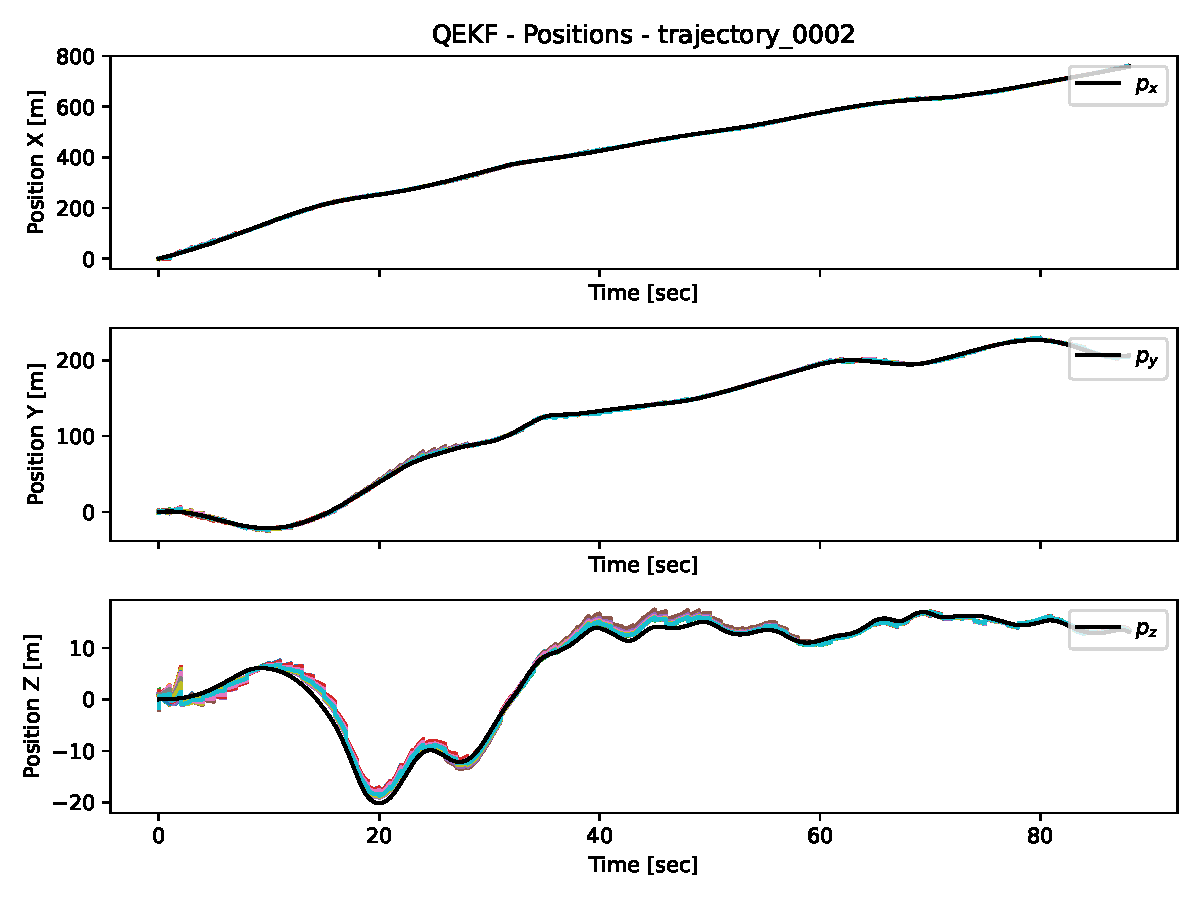
\includegraphics[width=0.8\textwidth]{figs/QEKF_trajectory_0002_positions.pdf}
    \caption{QEKF Position Monte Carlo Trials}
    \label{fig: QEKF Position Monte Carlo Trials}
\end{figure}

\begin{figure}[H]
    \centering
    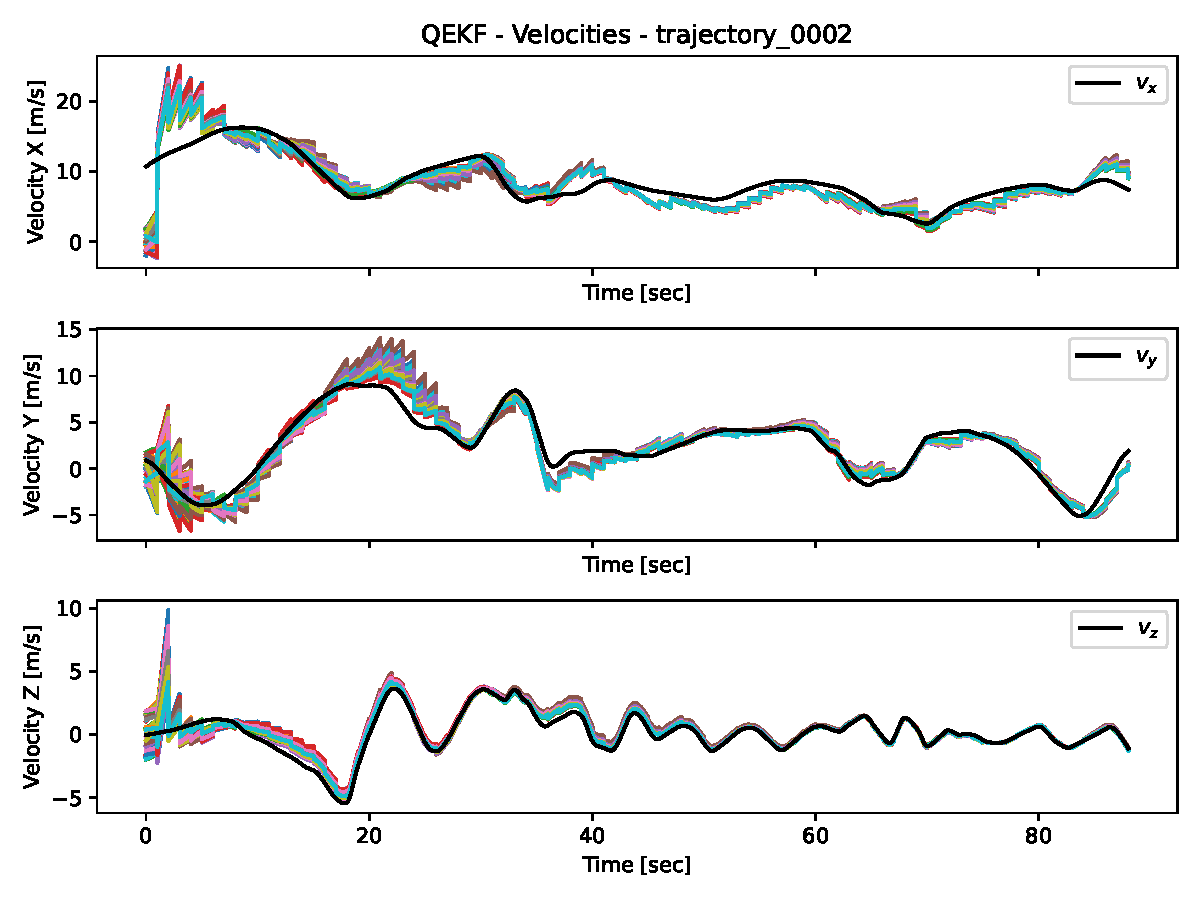
\includegraphics[width=0.8\textwidth]{figs/QEKF_trajectory_0002_velocities.pdf}
    \caption{QEKF Velocity Monte Carlo Trials}
    \label{fig: QEKF Velocity Monte Carlo Trials}
\end{figure}

\begin{figure}[H]
    \centering
    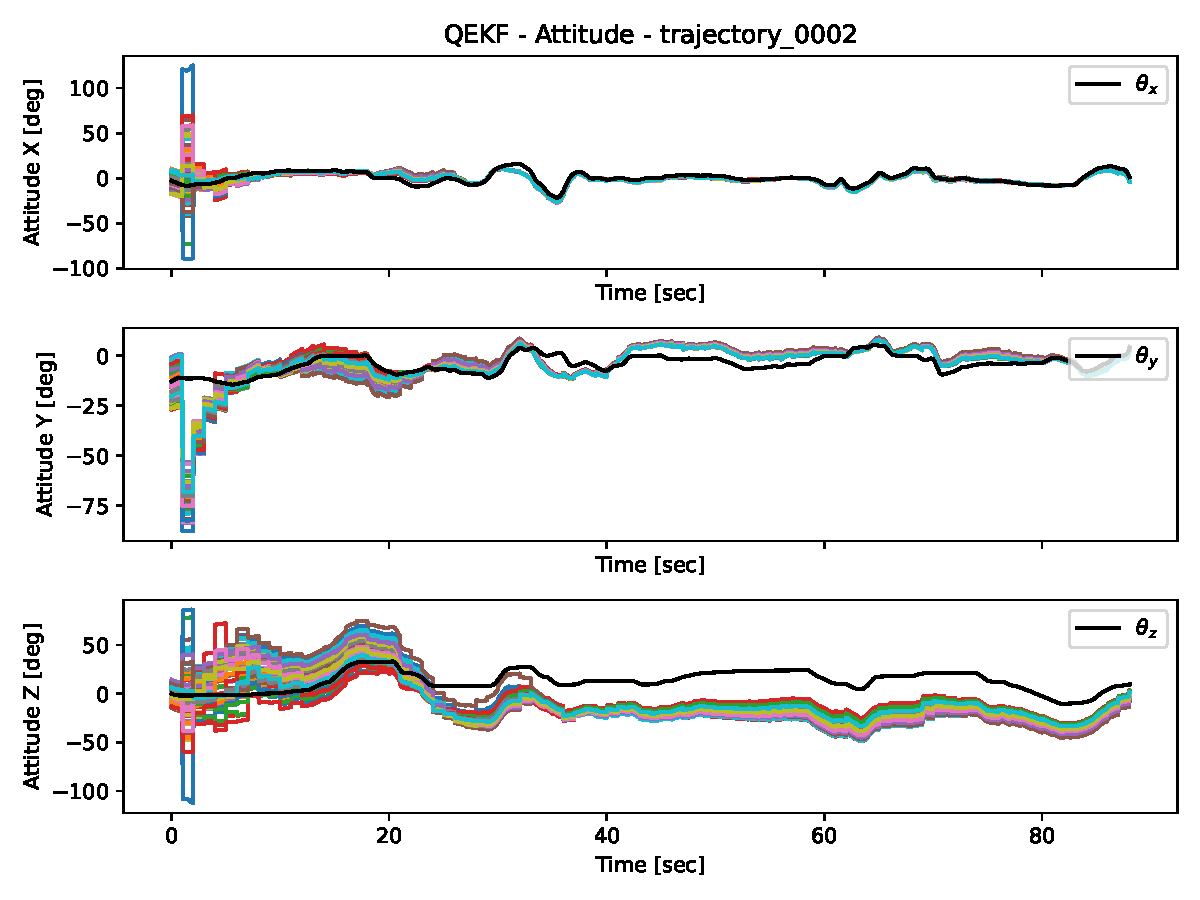
\includegraphics[width=0.8\textwidth]{figs/QEKF_trajectory_0002_attitudes.pdf}
    \caption{QEKF Attitude Monte Carlo Trials}
    \label{fig: QEKF Attitude Monte Carlo Trials}
\end{figure}

\begin{figure}[H]
    \centering
    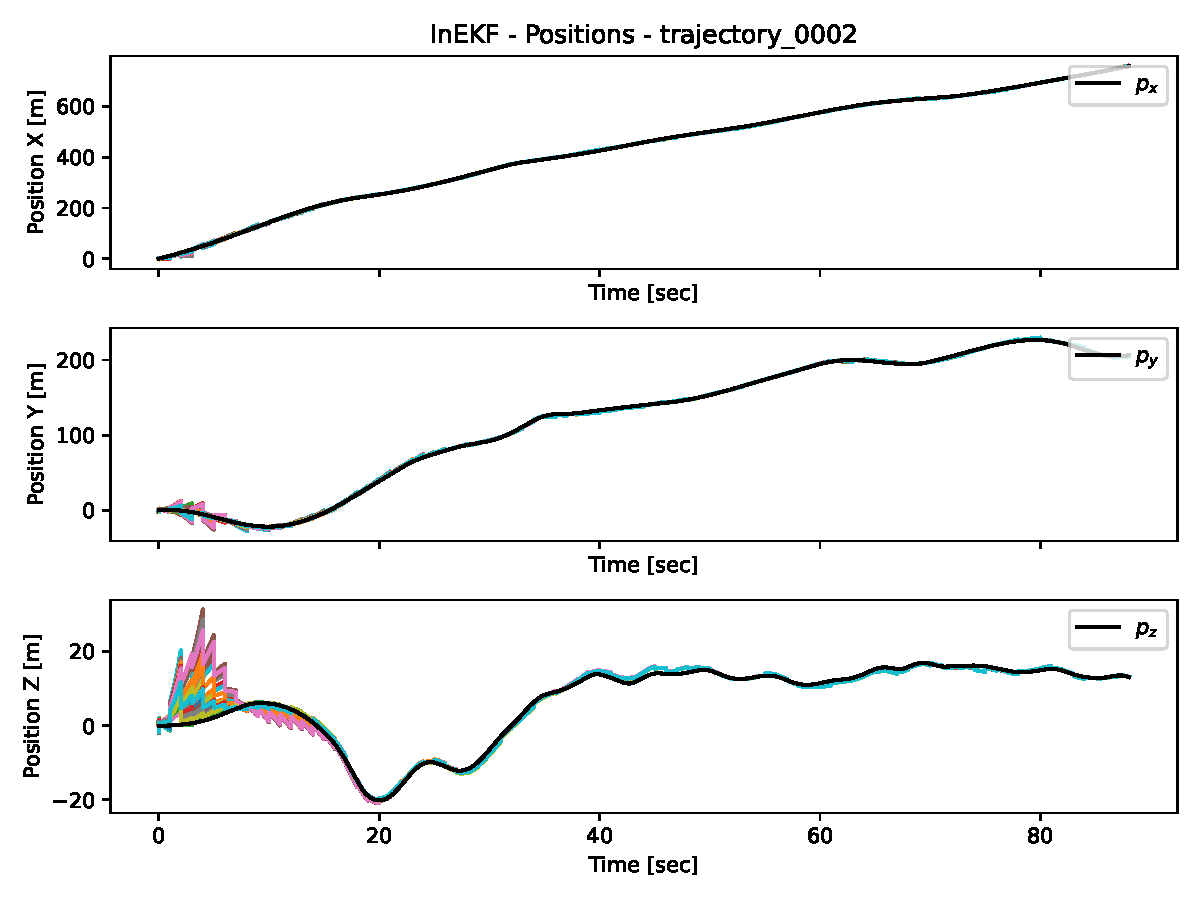
\includegraphics[width=0.8\textwidth]{figs/InEKF_trajectory_0002_positions.pdf}
    \caption{InEKF Position Monte Carlo Trials}
    \label{fig: InEKF Position Monte Carlo Trials}
\end{figure}

\begin{figure}[H]
    \centering
    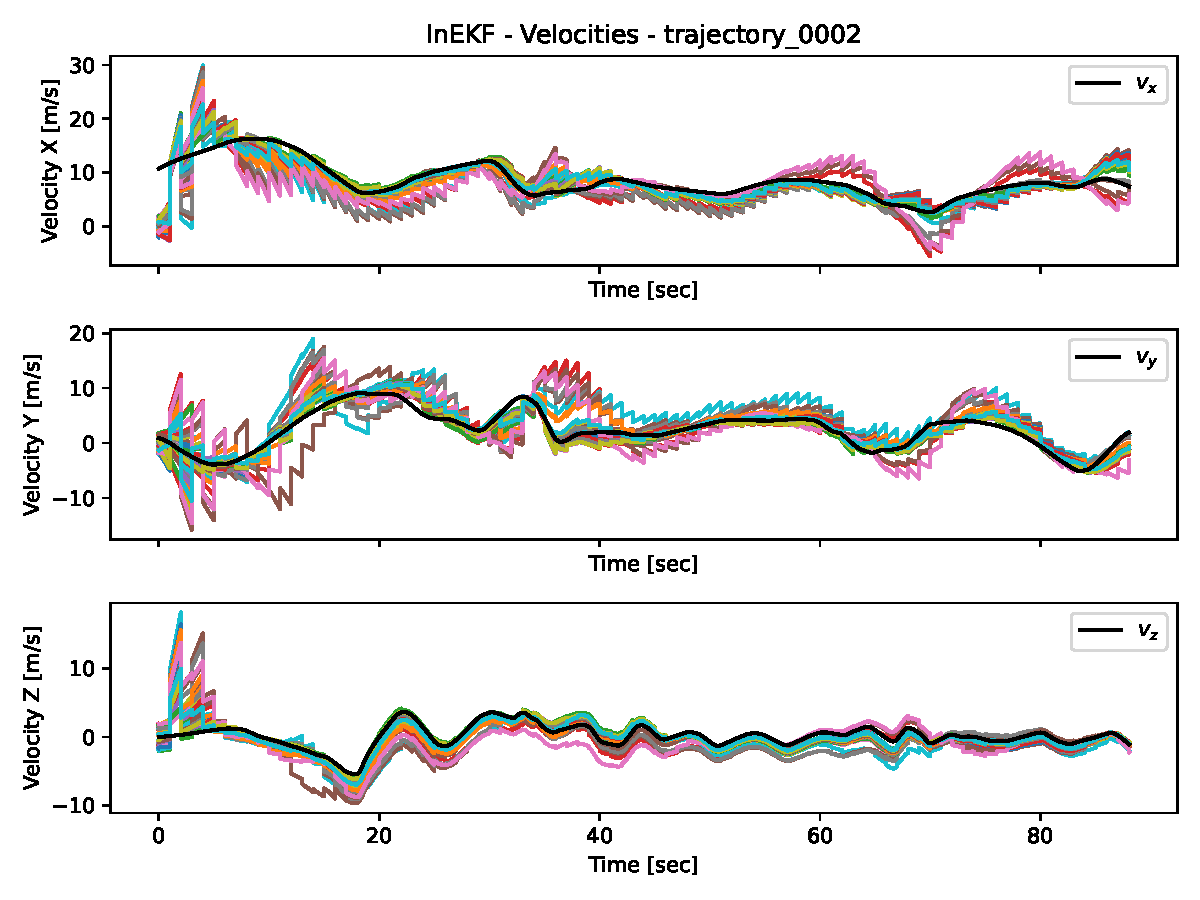
\includegraphics[width=0.8\textwidth]{figs/InEKF_trajectory_0002_velocities.pdf}
    \caption{InEKF Velocity Monte Carlo Trials}
    \label{fig: InEKF Velocity Monte Carlo Trials}
\end{figure}

\begin{figure}[H]
    \centering
    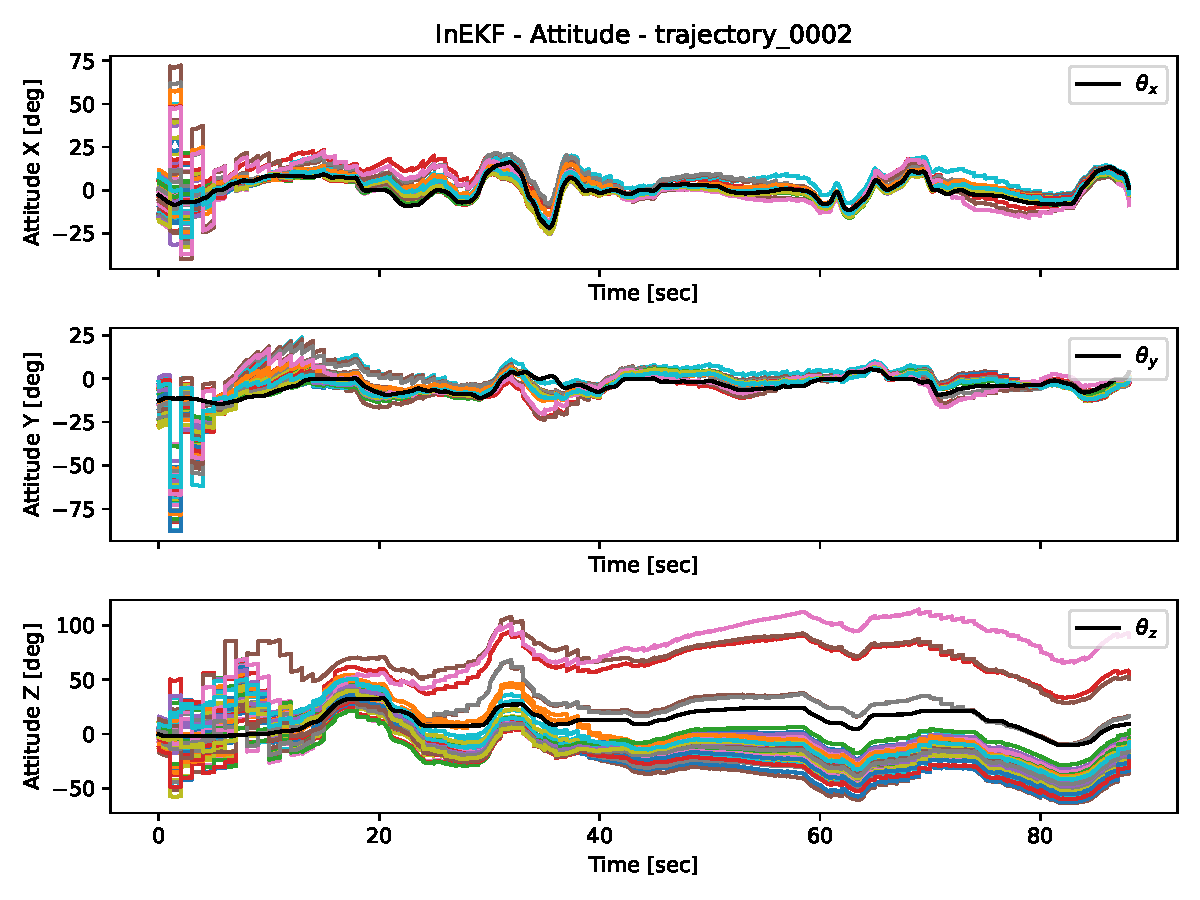
\includegraphics[width=0.8\textwidth]{figs/InEKF_trajectory_0002_attitudes.pdf}
    \caption{InEKF Attitude Monte Carlo Trials}
    \label{fig: InEKF Attitude Monte Carlo Trials}
\end{figure}

\begin{table}[H]
\centering
\begin{tabular}{|c|c|c|c|c|c|}
    \hline
    \textbf{States} & \multicolumn{4}{|c|}{\textbf{Error Metrics}} & \textbf{Units} \\
    \cline{2-5}
    & \textbf{Mean QEKF} & \textbf{Mean InEKF} & \textbf{Max QEKF} & \textbf{Max InEKF} & \\
    \hline
    Position X & 1.2989 & 1.2205 & 9.2388 & 9.2800 & $m$ \\
    Position Y & 0.8957 & 0.8579 & 4.5489 & 3.8393 & $m$ \\
    Position Z & 0.8720 & 0.8396 & 3.6690 & 11.6386 & $m$ \\
    \hline
    Velocity X & 1.4704 & 1.3089 & 10.8342 & 10.8531 & $\frac{m}{s}$ \\
    Velocity Y & 0.8594 & 0.7439 & 3.7589 & 3.1248 & $\frac{m}{s}$ \\
    Velocity Z & 0.3489 & 0.3536 & 5.8320 & 10.3547 & $\frac{m}{s}$ \\
    \hline
    Attitude X & 2.6254 & 2.2281 & 19.5816 & 18.0167 & $deg$ \\
    Attitude Y & 4.5363 & 4.0555 & 59.7614 & 52.4789 & $deg$ \\
    Attitude Z & 26.9152 & 23.6016 & 43.5164 & 53.0185 & $deg$ \\
    \hline
\end{tabular}
\caption{Monte Carlo Error Metrics for QEKF and InEKF Filters}
\label{tab: error metrics}
\end{table}



\subsection{Discussion}
Using just the GPS position measurement, it is clear that both QEKF and InEKF suffer from unobservability. This affects the bias states (not shown) and causes certain states such as the attitude in the Z direction to incurred large errors. By adding more measurements, observability can be improved and this issues can be reduced.

Despite this issue, the QEKF and InEKF results can still be compared. In the InEKF plots, it is clear that quicker convergence of the states does occur which was also found in \cite{Contact-Aided_Invarant_EKF} and \cite{9444664}. This can be most clearly seen the in the velocity and attitude plots. This is due to the InEKF linearization being more accurate and being less sensitive to the initial errors as compared to the QEKF. Comparing the mean errors, the InEKF performs slightly better than the QEKF in all states besides in the Z velocity. This gives further confidence that the Lie group representation of the state does improve results because the rotation, velocity, and position are not decoupled like in the QEKF. Overall, the differences between the two filters were minor when using only GPS measurements. However, initial results suggest that the InEKF may hold an advantage over the QEKF. Future work incorporating additional measurements into the system will help clarify the extent of this advantage.

%The purpose of these simulations was to in part determine how well the InEKF performed compared to the more standard QEKF filter. In the InEKF plots, it is clear that quick convergence of the states does not occur despite results found in \cite{Contact-Aided_Invarant_EKF} and \cite{9444664}. This can be attributed to several factors which highlight issues that occur when the theoretical advantages of the InEKF are no longer true. One cause is the bias augmentation to the InEKF. The InEKF needs to be linearized around the current state just like the QEKF due to the bias states. Therefore, having a bad initialization of the state does affect the filter because its error is no longer invariant. Another issue is the lack of observability due to only using GPS position measurement and structure of the state transition matrix. This unobservability affects the bias random walk states causing drift as well as the attitude states. Another issue with the InEKF is having to switch between the right and left InEKF filters which is not exact for the bias augmented system. While exact when just estimating the state defined for the Lie group \eqref{eq: SE3_2 group}, the inclusion the parameter bias vector means that each switch from the right propagation form to the left measurement form induces some error. 

%Directly comparing the two filters, the mean error in the position and velocity is relatively similar besides in the vertical z components where the QEKF performed considerably better than the InEKF. For the attitudes, the InEKF performs moderately better across all attitudes. The error is found to be much larger in the z attitude due to unobservability of the state, however, it is found that the error propagated for the z attitude is less for the InEKF. Overall, the differences between the two filters, within the constraints of this estimation problem, are not substantial enough to definitively conclude that one filter outperformed the other. Future simulations and modifications to the estimation problem, as mentioned in the conclusion section, could help differentiate which filter performs better.

%%%%%%%%%%%%%%%%%%%%%%%%%%%%%
%To do:
% -> Add comparision of uncertainty. Will need to reference first order approximation equations for InEKF
% -> Mention why biases are not plotted
% -> Mention observablility



% Initial covariance table
% \begin{table}[h!]
% \centering
% \begin{tabular}{|c|c|c|}
% \hline
% \textbf{State} & \textbf{Initial Standard Deviation ($\mathbf{R}^3$)} & \textbf{Units} \\ 
% \hline
% Position & $\sigma_{p} = 5$ & $m$\\ 
% \hline
% Velocity & $\sigma_{v} = 2$ & $\frac{m}{s}$\\  
% \hline
% Attitude & $\sigma_{\theta} = 7e-1$ & $rad$\\ 
% \hline
% Accelerometer Bias & $\sigma_{ba} = 1e-1$ & $\frac{m}{s^3}$ \\ 
% \hline
% Gyroscope Bias & $\sigma_{b \omega} = 1e-2$ & $\frac{rad}{s^2}$ \\ 
% \hline
% \end{tabular}
% \caption{QEKF Initial Covariance ($P_0$)}
% \label{tab: Initial Covariance}
% \end{table}
\section{Conclusion}
%%%%%%%%%%%%%%%%%%%%%%%%%%%%%

\subsection{Summary}
This report explored how the Quaternion Extended Kalman Filter and Invariant Extended Kalman Filter compared in a drone state estimation simulation. Detailed background was provided for the IMU, GPS, and magnetometer measurement models that were used to estimate the states of the drone. Background was then provided for both filters explaining the derivation of each filter for the estimation problem. A Monte Carlo simulation was then conducted for each filter. From the results, the overall error in the state estimates was found to be similar between the two filters. Marginal improvements in state convergence were found in the InEKF during an initial time period. Future work in expanding the Monte Carlo simulations and adding additional measurements will enhance the comparison of the two filters.


\subsection{Future Work}
There are multiple different ways this work could be improved in the future. The key improvements I would like to see worked are the following:
\begin{itemize}
    % \item Including a observability analysis for QEKF and InEKF to demonstrate which states are not observable
    \item Adding new measurements to the current system. Additional measurements could come from a barometer, air speed sensor and/or vision. For vision, the Mid-Air Dataset \cite{Fonder2019MidAir} provides various measurements such as stereo RGB pictures
    \item Including Monte Carlo simulations across different trajectories and randomize the noise separately for each trajectory
    \item Comparing body estimates of states could help give more insight into how the two filters compare. Currently, only the world frame estimate of the states are calculated
    \item Compare uncertainty estimates for each of the filters
    \item Give a example of the InEKF using a simple system to demonstrate the possible invariant properties and show what the covariance in the Lie group vs. Lie algebra looks like
    \item Include a tradition Kalman Filter that propagates the Euler angles without a quaternion or rotation matrix representation
    \item Create a C++ implementation of the filters
     \item Apply these filters to an actual drone
    \item Compare the computational time required to run each filter
    \item Include more background on the Lie groups and Lie algebra including visuals
    \item Add some of the missing proofs that are mentioned in the background sections for each filter
    \item Better characterize with numbers what it means to be converged
\end{itemize}

\clearpage
%%%%%%%%%%%%%%%%%%%%%%%%%%%%%


% References setup
\bibliographystyle{alpha}
\bibliography{refs}

\end{document}
%%%%%%%%%%%%%%%%%%%%%%%%%%%%%



% Notes:
To comment out text ctrl+shift+7

